%%%%%%%%%%%%%%%%%%%%%%%%%%%%%%%%%%%%%%%%%%%%%%%%%%%%%%%%%%
%
% Vzor pro sazbu kvalifikační práce
%
% Západočeská univerzita v Plzni
% Fakulta aplikovaných věd
% Katedra informatiky a výpočetní techniky
%
% Petr Lobaz, lobaz@kiv.zcu.cz, 2016/03/14
%
%%%%%%%%%%%%%%%%%%%%%%%%%%%%%%%%%%%%%%%%%%%%%%%%%%%%%%%%%%

% Možné jazyky práce: czech, english
% Možné typy práce: BP (bakalářská), DP (diplomová)
\documentclass[czech,DP]{thesiskiv}

% Definujte údaje pro vstupní strany
%
% Jméno a příjmení; kvůli textu prohlášení určete, 
% zda jde o mužské, nebo ženské jméno.
\author{Kateřina Kratochvílová}
\declarationfemale

%alternativa: 
%\declarationfemale

% Název práce
\title{Nástroj pro automatickou identifikaci KIR alel}

\thanktext{Ráda bych poděkovala Ing. Lucii Houdové, Ph.D. za cenné rady, věcné připomínky, trpělivost a ochotu, kterou mi v průběhu zpracování této práce věnovala. Dále bych chtěla poděkovat panu ing. Jiřímu Fatkovi za jeho rady a pomoc při vytváření praktické části. }
% 
% Texty abstraktů (anglicky, česky)
%
\abstracttexten{The text of the abstract (in English). It contains the English translation of the thesis title and a short description of the thesis.
Text abstraktu (česky). Obsahuje krátkou anotaci (cca 10 řádek) v češtině. Budete ji potřebovat i při vyplňování údajů o bakalářské práci ve STAGu. Český i anglický abstrakt by měly být na stejné stránce a měly by si obsahem co možná nejvíce odpovídat (samozřejmě není možný doslovný překlad!).}

\abstracttextcz{Diplomová práce se zabývá identifikací KIR alel. Cílem práce je vytvořit nástroj pro jejich automatickou identifikaci. V práci byli rozebrány metody získávaní dat z DNA, konkrétně next-generation sequencing (NGS) a dále analyzovány bioinformatické nástoje ART a Bowtie. Nástoj byl vyvíjen na syntetických readech vytvořených pomocí nástroje ART a nakonec testován na datech získaných z FN Plzeň případně z BC LF UK Plzeň. 

}

% Na titulní stranu a do textu prohlášení se automaticky vkládá 
% aktuální rok, resp. datum. Můžete je změnit:
%\titlepageyear{2016}
%\declarationdate{1. března 2016}

% Ve zvláštních případech je možné ovlivnit i ostatní texty:
%
%\university{Západočeská univerzita v Plzni}
%\faculty{Fakulta aplikovaných věd}
%\department{Katedra informatiky a výpočetní techniky}
%\subject{Bakalářská práce}
%\titlepagetown{Plzeň}
%\declarationtown{Plzni}

%%%%%%%%%%%%%%%%%%%%%%%%%%%%%%%%%%%%%%%%%%%%%%%%%%%%%%%%%%
%
% DODATEČNÉ BALÍČKY PRO SAZBU
% Jejich užívání či neužívání záleží na libovůli autora 
% práce
%
%%%%%%%%%%%%%%%%%%%%%%%%%%%%%%%%%%%%%%%%%%%%%%%%%%%%%%%%%%

% Zařadit literaturu do obsahu
\usepackage[nottoc,notlot,notlof]{tocbibind}

% Umožňuje vkládání obrázků
\usepackage[pdftex]{graphicx}

\usepackage{subcaption}
% Odkazy v PDF jsou aktivní; navíc se automaticky vkládá
% balíček 'url', který umožňuje např. dělení slov
% uvnitř URL
\usepackage[pdftex]{hyperref}
\hypersetup{colorlinks=true,
  unicode=true,
  linkcolor=black,
  citecolor=black,
  urlcolor=black,
  bookmarksopen=true}

% matematicke rovnice %
\usepackage{amsmath}
\usepackage{fancyhdr}
\usepackage{float}
\numberwithin{equation}{section}
% Při používání citačního stylu csplainnatkiv
% (odvozen z csplainnat, http://repo.or.cz/w/csplainnat.git)
% lze snadno modifikovat vzhled citací v textu
\usepackage[numbers,sort&compress]{natbib}

\usepackage{multirow}

%pouzite zkratky
\usepackage{blindtext}
\usepackage{scrextend}
\addtokomafont{labelinglabel}{\sffamily}

%%%%%%%%%%%%%%%%%%%%%%%%%%%%%%%%%%%%%%%%%%%%%%%%%%%%%%%%%%
%
% VLASTNÍ TEXT PRÁCE
%
%%%%%%%%%%%%%%%%%%%%%%%%%%%%%%%%%%%%%%%%%%%%%%%%%%%%%%%%%%
\begin{document}
%
\maketitle
\tableofcontents

\chapter{Úvod}
Transplantace krvetvorných buněk se využívá jako terapeutická procedura pro mnoho vážných hematologických poruch mezi které patří například akutní myeloidní leukemie. Transplantace jako taková je poměrně jednoduchý proces, kdy jsou dárci odebrány krvetvorné buňky a vpraveny do těla pacienta trpícím hematologickou poruchou. Problém nastává při reakci imunitního systému na nově vložený štěp. V případě, že si štěp s imunitním systémem nebudou rozumět, může dojít k silné zánětlivé reakci, která může skončit až smrtí pacienta. 
\\
\\
K potlačení odmítnutí se vybírají dárci podle shody v HLA znacích, věku a pohlaví. Ovšem ani to neni bezrizikové. V poslední době se množí studie, které prokazují vliv takzvaných non-HLA genů. Jedním z nich může být i gen Killer-cell immunoglobulin-like receptor (KIR). V případě, kdy by se rozhodovalo mezi více dárce by se mohl ten vhodnější vybrat právě na základě KIR. Pro zjištění jak HLA znaků tak KIR genů se využívají sekvenační metody. \citep{KIR_transplantace_jindra} 
\\
\\
Cílem práce je navrhnout a implementovat nástroj pro automatickou identifikaci KIR alel. Vstupní data tzv. ready jsou neznámý kus DNA (posloupnost písmen A, C, G a T) a jsou výstupem ze sekvenačních metod. Tyto data budou pro vývoj nástroje simulována nástrojem ART a v konečné fázi testování budou data vyměněna za data z FN Plzeň. Jelikož je třeba odhadnout co se pod danou posloupností nachází, bude použit nástroj bowtie2 pro zarování readů vzhledem k referenčním KIR genům. V poslední fázi bude vyhodnocena shoda readů a referenčních genů.

\chapter{Imunitní systém a jeho spojitost s geny}
\section{Geny}
V každé buňce lidského organismu, konkrétně v buněčném jádře, je možné nálest 46 chromozomů. Jeden chromozom představuje stočenou dlouhou molekulu DNA (Deoxyribonuklenovou kyselinu). Všech 46 chromozomů obsahuje okolo 100 000 genů. Drobný segment DNA, který řídí buněčnou funkci je právě gen. Konkrétní forma genu je alela. \citep{en_smith}

\begin{figure}[H]		
		\centering
		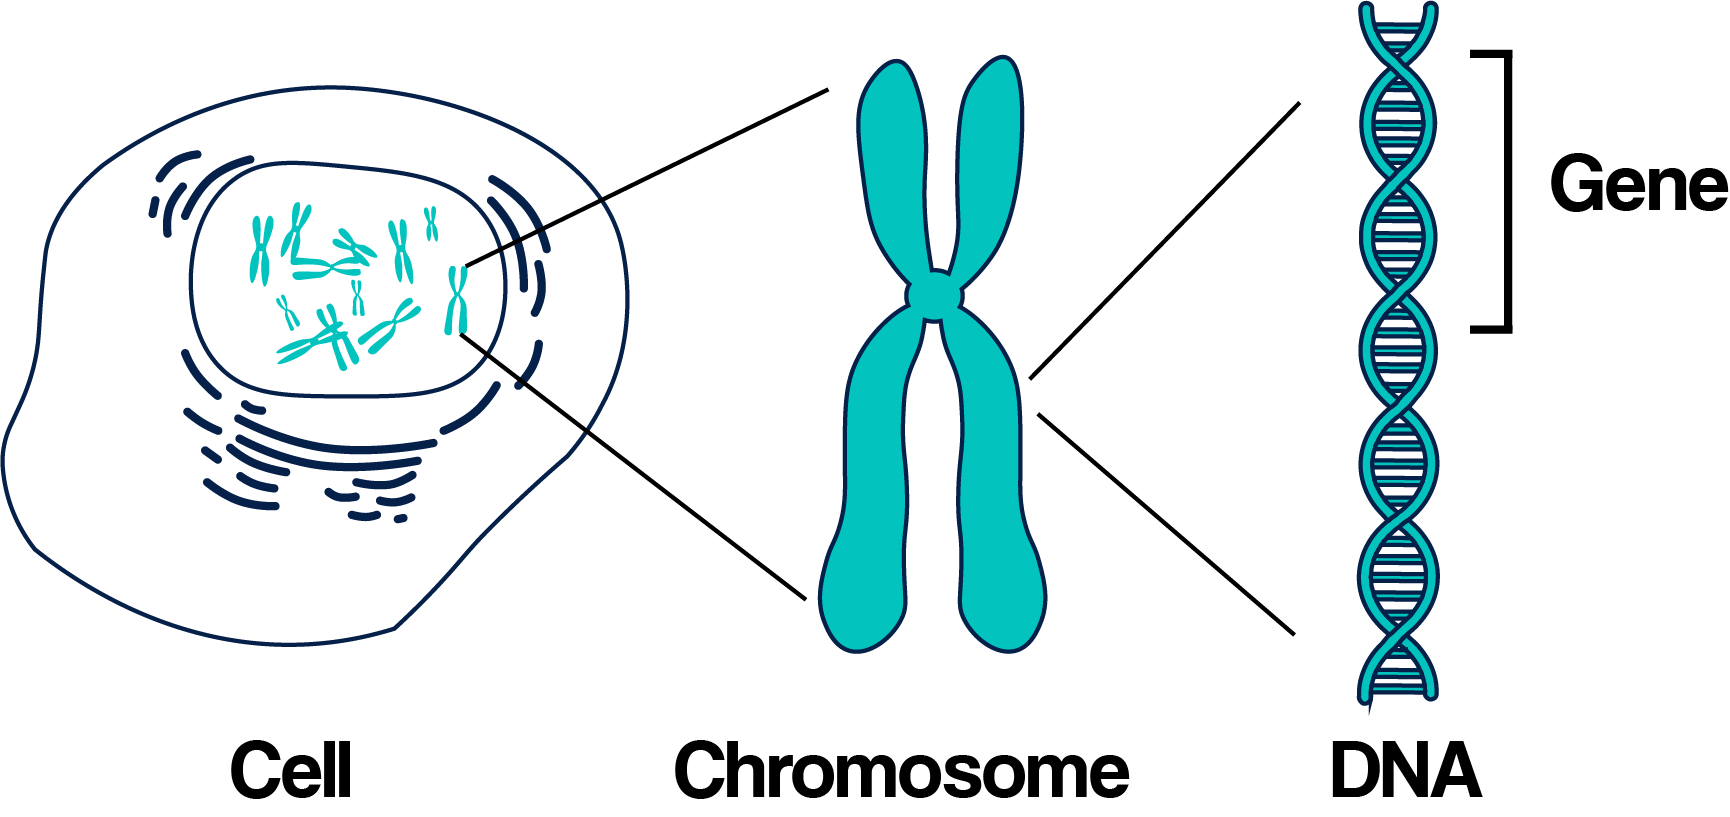
\includegraphics[width=150px]{./img/lidska_bunka.png}
		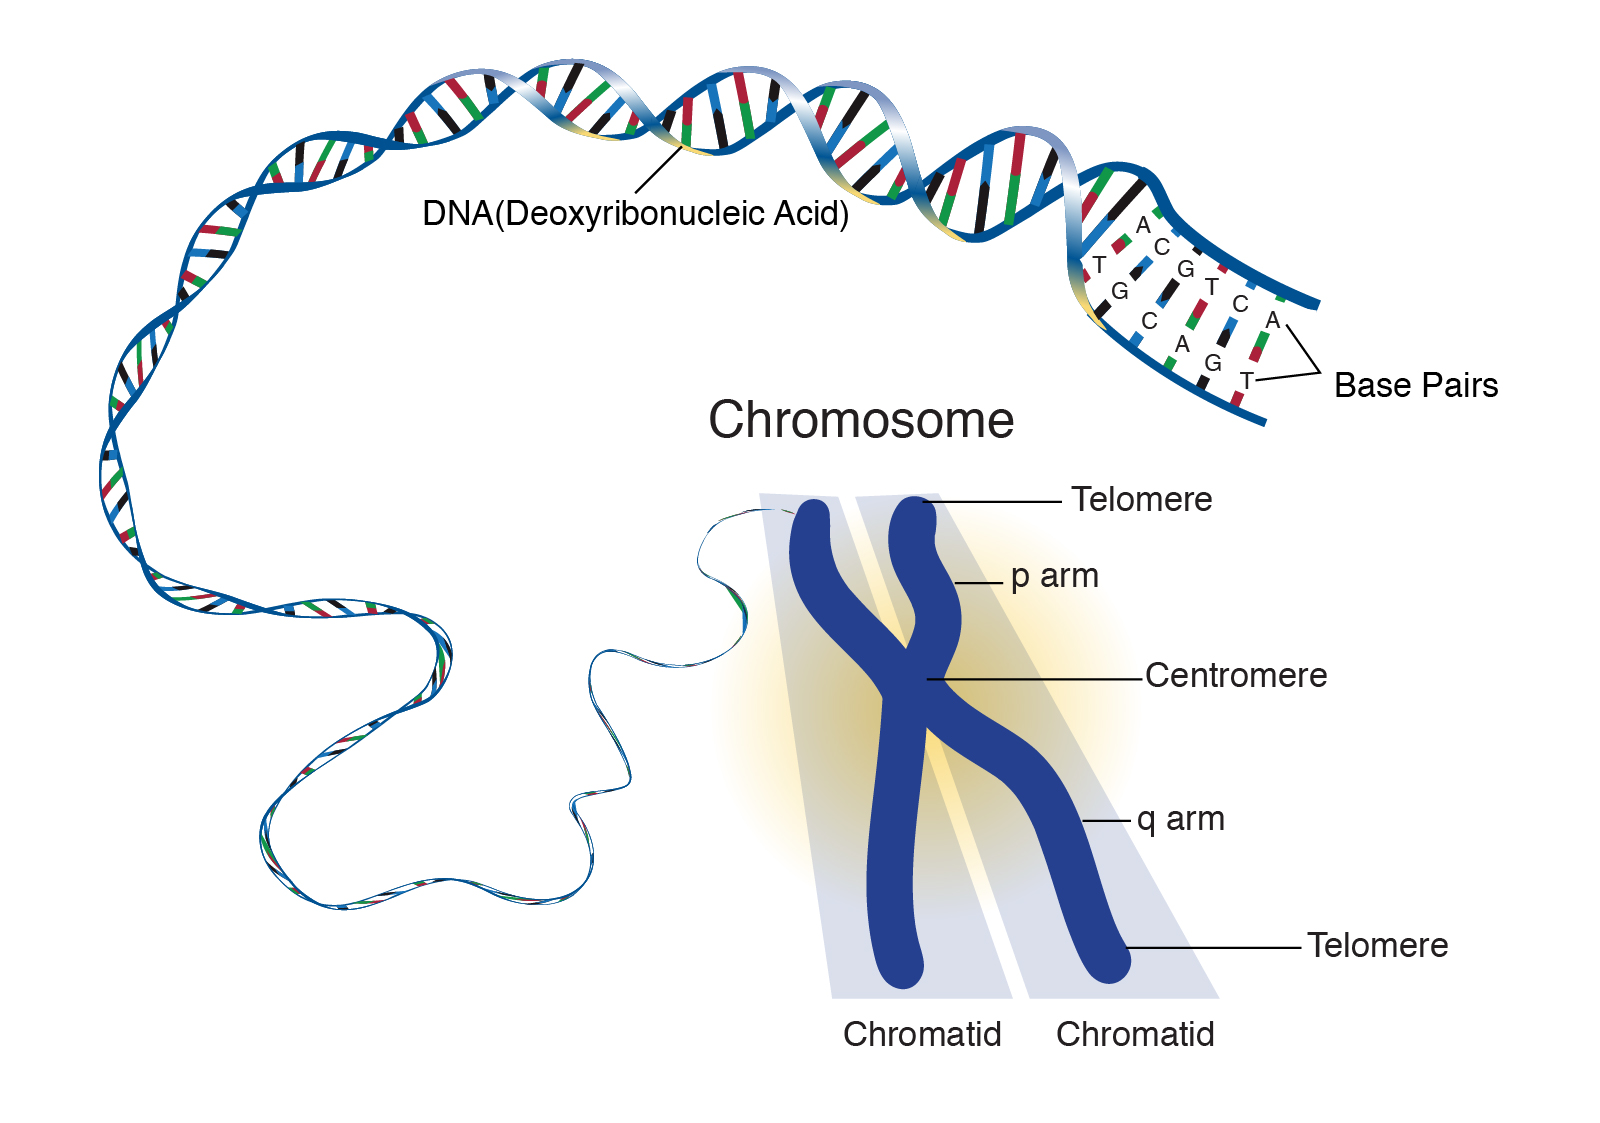
\includegraphics[width=200px]{./img/chromosome.jpg}
		\caption{Převzato z \cite{human_cell} a \cite{chromosome_structure}}
		\label{fig:chrmosome}
\end{figure}

\noindent
Uvnitř buňky máme celý genom který se ovšem nemusí projevit na povrchu buňky. Pokud se vlastnost kterou gen přenáší projeví na povrchu buňky označujeme to jako exprese genu (jeho sebevyjádření). Od toho se odvíjí i konkrétní názvosloví typu KIR gen, KIR receptor či molekula.


\section{Imunitní systém}
Imunitní systém chrání organismus před škodlivinami. Skládá se ze dvou hlavních částí vrozené imunity a získané imunity. Reakce imunitního systému je vždy komplexní reakce organismu mezi jednotlivými buňkami imunitního systému reagující na přítomnost specifických antigenů. Antigeny jsou látky, které imunitní systém rozpozná a zareaguje na ně. V podstatě to může být jakákoli bílkoviná sloučenina. Antigen se obvykle nachází na povrchu buňky jako vyjádření genu. Imunitní systém následně zjistí o jaký antigen se jedná, respektivě o jakou buňku se jedná, zda tělu vlastní (např. zdravá buňka) nebo buňku tělu cizí (např. nádorová buňka), tedy jedná-li se o expresy lidského genu nebo například viru. Jedná-li se o buňku tělu cizí imunitní systém reaguje snahou ji zničit. 
\\
\\
\textbf{Vrozená imunita} též označována přirozená, neadaptivní, antigenně nespecifická je neměnně zapsána v DNA. To znamená, že při každém setkání s antigenem odpoví stejnou reakcí. Buňky nesoucí vrozenou imunitu jsou stále přítomně v krvy, takže jejich případná aktivace je takřka okamžitá (minuty až hodiny). Do této imunity patří i natural killer buňky s KIR receptory, které budou dále rozebírány v textu. 
\\
\\
\textbf{Získaná imunita} též označována specifická či adaptivní oproti specifické má v genomu zapsány pouze své základy. V průběhu lidského života se vyvyjí a mění. Změna může nastat například očkování nebo proděláním patřičné choroby. Tato změna ovšem nemusí být trvalá. Z těchto důvodů může být odpověď ziskáné imunity při setkání se stejnou chorobou rozdílná. Fungování získané imunity zajišťují T- a B- lymfocyty, ale nefunguje samostantně. Při zabíjení patogenů spolupracuje s vrozenou imunitou.


\section{HLA a non-HLA geny}
Human leucocyte antigen (HLA) je genetický systém, který je primárně zodpovědný za rozeznávání vlastního od cizorodého. Někdy je termín HLA zaměňován s MHC. MHC (Major histocompatibility complex) je souhrný termín pro všechny komplexy, kdy podskupinou jsou práve HLA (H - Human) který je pro lidi. Stejně tak existuje DLA (D - Dog) který je pro psy. Z funkčního i biologického hlediska jde však u všech savců o stejnou skupinu genů. \cite{KIR_transplantace_jindra}
\\
\\
Přesná definice mezi HLA a non-HLA geny neexistuje. Mimo jiné i jejich rozdělení není v literaturách sjednocené. Jak je vidět z obrázku \ref{fig:hla_genome} je možné geny rozdělit do tří tříd. V některých literaturach je možné nalést označení non-HLA genů jako geny III.třídy v jiné, že jsou to všechny geny III třídy a některé geny třídy I. Tato práce se bude v označení za gen non-HLA či HLA odkazovat na hla.alleles \cite{imgt_hla_database}. Zjednodušeně tedy můžeme říci, že geny které nejsou řazeny k HLA skupinám jsou non-HLA. Je-li gen označen za non-HLA neznamená to, že by neměl souvislost s funkcí imunitního systému. Naopak má, jen ne výlučně s HLA systémem. Non-HLA geny kódují produkty spojené s imunitními procesy. Mezi non-HLA geny mimo jiné patří MICA, MICB a KIR. \cite{imgt_hla_database}

\begin{figure}[H]		
		\centering
		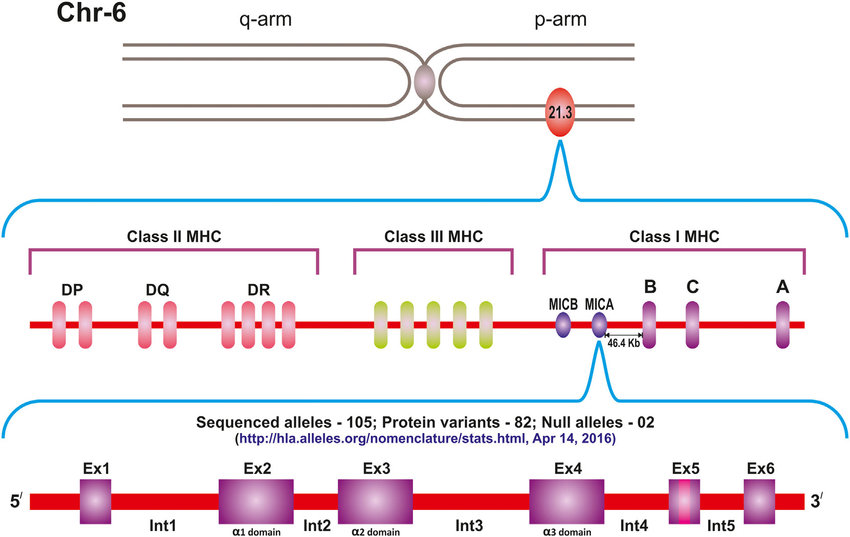
\includegraphics[width=300px]{./img/genom6_mica.jpg}
		\caption{Šestý chromozom zobrazující HLA i non-HLA geny. Protein vzniklý expresí MICA genu je definován exony, které definují přepis do RNA. Introny v praxi nehrají roli a často jsou sekvenovány jen exony. \cite{chromozome6_mica} 
		}
		\label{fig:hla_genome}
\end{figure}

\noindent
HLA a některé non-HLA geny se nacházejí na krátkém raménku 6 chromozomu, konkrétně 6p21.3 a zaujímá úsek přibližně jednu tisícinu genomu. Tento region je nejvíce komplexní a polymorfní na lidském genomu s více než 220 geny. Oproti tomu jedna ze skupin non-HLA genů, konkrétně KIR geny, se nachází na 19 chromozomu. Rozsáhlá diverzita genů vznikala snahou eliminovat neustále se měnící spektrum patogenů. Produkty těchto genů na povrch buňky významně ovlivňují odpověď na infekční choroby a výsledky buněčné či orgánové transplantace. \cite{imgt_hla_database}
 

\subsection{Alela a gen}
Alelu můžeme definovat jako variantu genu s nepatrným rozdílemem v sekvenci nukleotidů DNA oproti jiné alele stejného genu. Geny se vyskytují minimálně ve dvou formách (dvou alelách), mnohdy jich, ale může být více. U jednoho člověka můžou být přítomny pouze dvě rozdílné alely daného genu. Gen určuje výskyt nějaké vlastnosti, například tento živočich bude mít oči. Alela pak určuje jakou barvu budou mít.
\\
\\
V případě genu KIR2DL1 mohou být jeho alely 0010101 a 0010102. Zápis genů tak, jak s nimi budeme pracovat může vypadat způsobem zobrazeným v \ref{alela_gen_prikad}. 

\begin{equation}\begin{split} 
   \label{alela_gen_prikad}
   		>KIR:KIR00001\: KIR2DL1*0010101\: 14738\: bp \\
		GTTCGGGAGGTTGGATCTCAGACGTG...
\end{split}\end{equation}

\noindent 
Označení $KIR:KIR0001$ označuje pořadové číslo, kdy alela byla nalezena. Oproti tomu $KIR2DL1*0010101$ je označení genu podle jeho vlastnotí.
\\
\\ 
TODO: Když najdu novou sekvenci tak kde je rozdíl jestli je to nový gen nebo nová alela? Neni to tak že na daný pozici v genomu je vždycky gen.. a alela určuje tu vlastnost? A na co je mi teda lotus? 
geny jsou již plně definované - The Human Genome Project (HGP) https://www.genome.gov/human-genome-project/What (geny jsou ty 2DL1, 3DL1....)

jde o nové varianty - alelické skupiny, konkrétní alely - to je ve vazbě na to, jakej protein je kódován
\\
\\
TODO tohle je asi jen HLA nevím jestli existuje něco jako obecné rozdělení genu a aleli, možná že rozdíl bude jen v tom že těch čísel pak může být za hvězdičkou několik v závislosti o alelu jaké skupiny genů se jedná
Aleli jdou definovány HLA-DRB1* což označuje označuje lokus, následované 4 čísly. 
TODO nevím jestli mám nějak rozebírat to že je tam HLA-DRB1 že tam je tam jednička na konci, já totiž nevím co to znamená
\\
\\
TODO tohle nevím jestli tam dávat: 
Alela zajišťuje konkrétní fenotypový projev genu. U jedince mohou na homologních jaderných chromozomech být přítomny pouze dvě alely. Když jsou v párových lokusech obě alely shodné, jde buď o dominantního homozygota (AA) nebo o recesivního homozygota (aa). Když jsou na párových chromozomech v daném lokusu přítomny různé alely, jde o heterozygota (Aa). Značení alel vzniká dohodou.




\section{Natural killer a jeho receptory}
\subsection{Natural killer}
Natural killer buňky (NK buňky) jsou velké granulární lymfocyty vrozeného imunitního systému. V krevním oběhu lidského těla je jich možné nalést $10-15\%$. Klíčovou vlastností NK buněk je nejenom schopnost rozlišit poškozené buňky od zdravích, ale i poškozené buňky rychle a efektivně likvidovat. Poškozené buňky mohou být buňky infokované virem či buňky transfomované v nádorové. Na povrchu NK buňky se nachází receptory, které jsou zobrazeny na obrázku \ref{fig:NK_receptors}, regulující odpověď imunitního systému. Natural killer buňky oproti B- a T- lymfocitům (buňkám získané imunity) nemají antigenně specifické receptory. Jedním ze způsobů jak NK buňky rozpoznávají a zabíjejí poškozené buňky je na základě interakce mezi KIR receptorem a HLA molekulou na povrchu zkoumané buňky (podrobněji viz sekce KIR). Stejně tak mohou zabíjet na základě receptoru NKG2D, který aktivuje cytoxickou reakci při setkání s ligandem MICA a MICB. Ligandem označujeme malou molekulu, která se váže na vazebné místo cílového proteinu(receptoru) a vyvolává fyziologickou odpověď která může mít inihiční či aktivační charakter. 
% https://www.khanacademy.org/science/biology/cell-signaling/mechanisms-of-cell-signaling/a/signal-perception
\begin{figure}[H]		
		\centering
		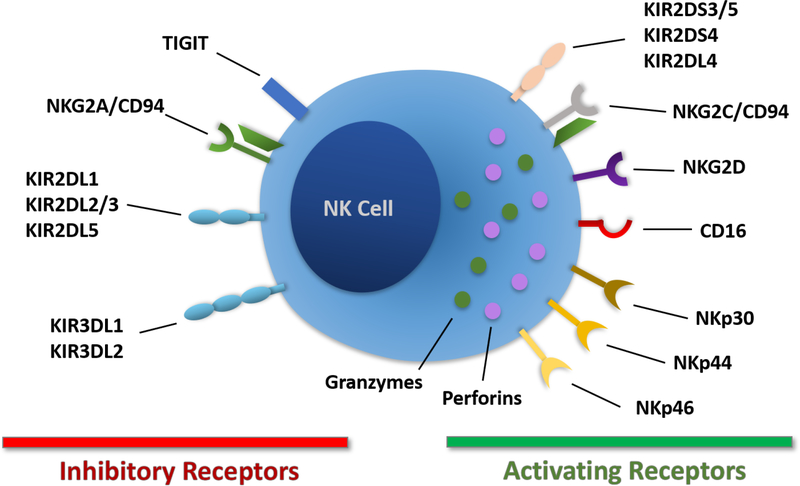
\includegraphics[width=300px]{./img/nk_receptory.jpg}
		\caption{Natural killer buňka a její receptory, rozděleny na aktivační a inhibiční. Pro tuto práci jsou důležité hlavně KIR receptory a NKG2D. \cite{NK_receptors} }
		\label{fig:NK_receptors}
\end{figure}

\subsection{NKG2D receptor}
NKG2D je jeden z nejvýznamnějších aktivačních receptorů na NK buňce rozpoznávající především buněčný stres, který může spustit cytotoxicitu (shopnost níčit buňky) i když se na povrchu buňky nachází inhibiční HLA-I ligandy.  
\\
\\
Geny skupiny MICA a MICB jsou označeny jako class I chain-related gene. To znamená, že se běžně neřadí do I. třídy MHC. Takto označované geny mají souvislost s MHC I třídy, ale narozdíl od nich neváží peptidy. Oproti HLA genům, které mají svoje produkty na lymfocytech, se produkty MICA a MICB nachází na epitelových buňkách. Nejedná se tedy o standardní HLA geny, proto jsou nověji v literaturách označovány jako non-HLA. Jejich expresí na povrch buňky jsou ligandy, které se váží na receptor NKG2D. Buňky s ligandy MICA a MICB se množí při nádorovém onemocnění, zanětu nebo pod vlivem různých forem buněčného stresu a díky navázáním na receptor může být spuštěna imunitní reakce. \cite{transfuzni_lekarstvi} \cite{MIC} \cite{NK_receptors} \cite{imgt_hla_database}


\subsection{KIR receptor}
Killer immunoglobulin-like receptor (KIR) je skupina genů řazených mezi non-HLA geny. Jejich zvláštností je fakt, že se nenachází na 6 chromozomu, ale na 19 a tak shodní dárci HLA znaků mohou být neshodní v KIR znacích. Jejich expresí jsou receptory na povrchu natural killer buněk. Dnes je známo 15 genů a 2 pseudogeny rozlišujících se na inhibiční a aktivační na základě cytoplasmatického ocásku a počtu imunoglobulínových domén. \citep{KIR_transplantace_jindra}

\begin{figure}[H]		
		\centering
		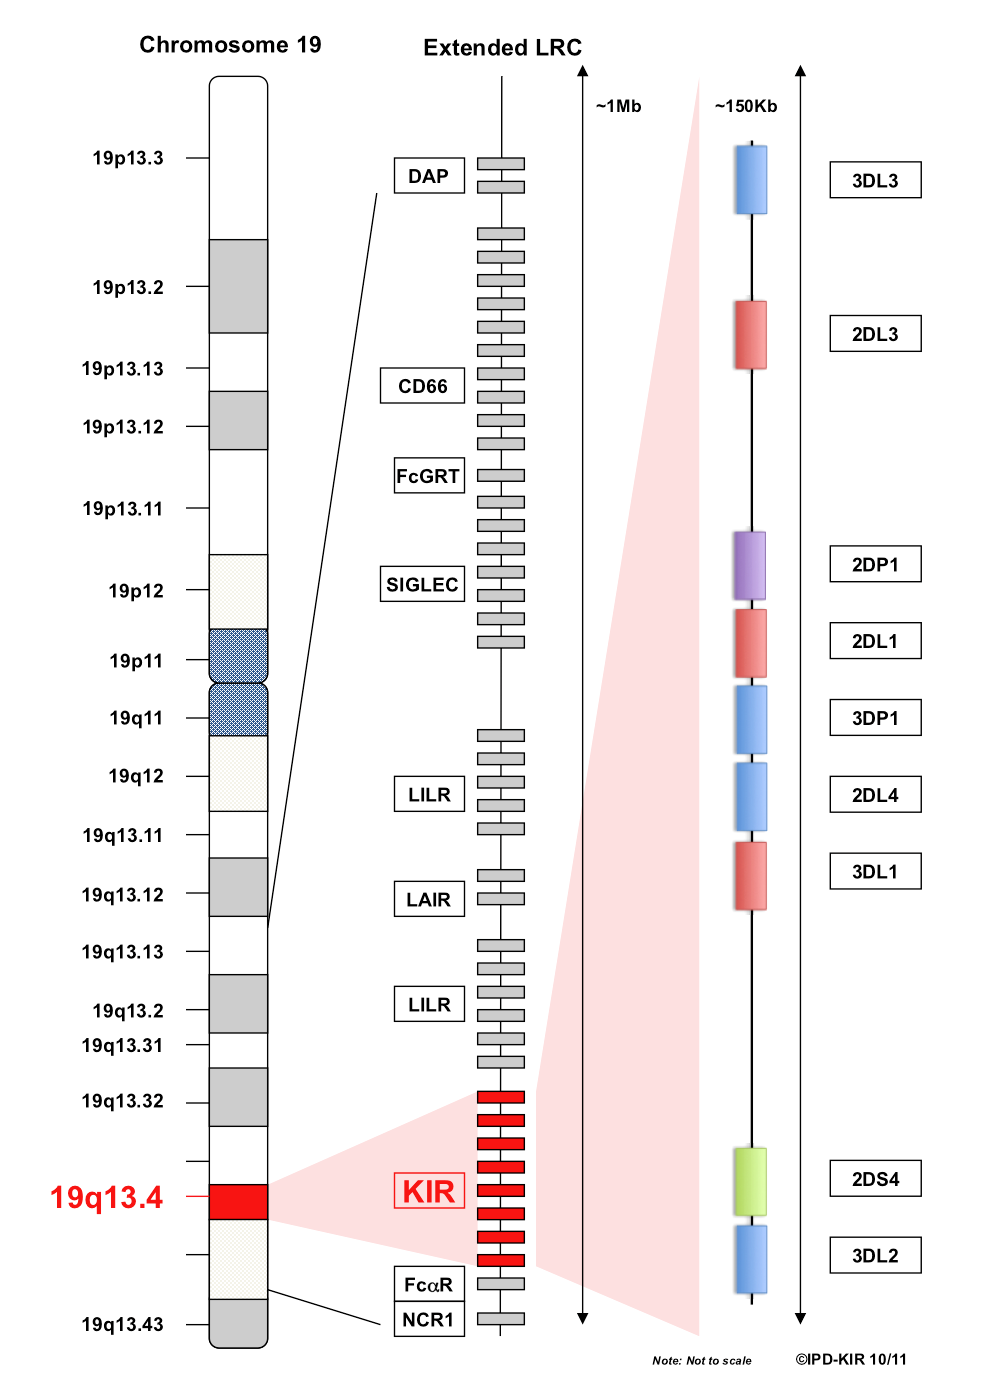
\includegraphics[width=250px]{./img/kir_pozice.png}
		\caption{KIR se nachází na 19 chromozomu v oblásni jménem leukocyte receptor complex (LRC). \cite{imgt_hla_database}}
		\label{fig:kir_position}
\end{figure}

\subsubsection{Nomenklatura KIR genů}
KIR geny (na obrázku \ref{fig:img_kir_nomenklatura}) se liší různou délkou cytoplasmatických ocásku (tail) a různým počtem imunoglobulin-like domén (lg-like). Na základě této rozmanitosti byla založena nomenklatura KIR genů, tedy jejich pojmenování. 
\\
\\
Jak je vidět na obrázku~\ref{fig:img_kir_nomenklatura}, cytoplasmatický ocásek může být dlouhý (long~-~L) nebo krátký (short~-~S). Oproti tomu imunoglubulínové domény se mohou vyskytovat 2~(2D) nebo 3~(3D). Právě z těchto vlastností vychází základ pojmenování KIR genů. Příkladem může být KIR2DL1*010101, kde 2D označuje dvě imunoglubulinové domény, L značí dlouhý ocásek, 1 značí že je to první 2DL protein. Následuje hvězdička oddělující gen od alely. První tři čísla označují alely, které se liší v sekvencích jejich kódovaných proteinů, další dvě číslice se používají k rozlišení alel, které se liší synonymnními rozdíly v kódující sekvenci. Konečné dvě cifry rozlišují alely na základě substituce v intronu, promotoru nebo jiné nekódující oblasti. \cite{imgt_hla_database}

\begin{figure}[H]		
		\centering
		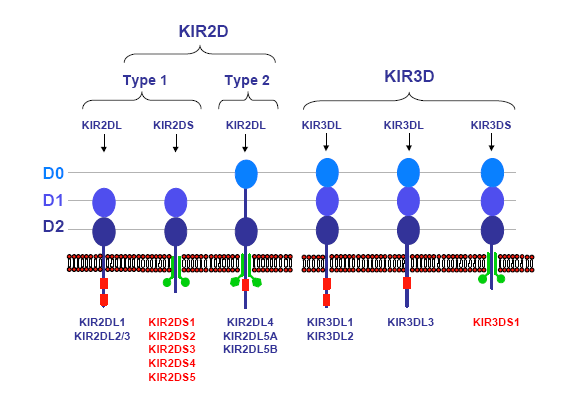
\includegraphics[width=\textwidth]{./img/KIR_nomenklatura.png}
		\caption{Nomenklatura KIR genů. \cite{KIR_transplantace_jindra}}
		\label{fig:img_kir_nomenklatura}
\end{figure}

\noindent
Další rozdělení KIR genů je již výše zmíněné inhibiční a aktivační. Na obrázku~\ref{fig:img_kir_nomenklatura} je možné si povšimnout detailu, že až na KIR2DL4 jsou aktivační KIR s krátkým ocáskem, zatímco inhibiční jsou s dlouhým ocáskem. 

\subsubsection{Aktivace NK buněk pomocí KIR}
Jak již bylo výše zmíněno KIR receptory můžeme rozdělit na inhibiční a aktivační. Zda dojde k aktivaci NK buňky rozhoduje právě jejich rovnováha na zkoumané buňce. Zatímco inhibiční receptory se váží hlavně na molekuly HLA, aktivační receptory rozpoznávají molekuly které jsou exprimovány na membránu při buněčném stresu. Obrázek \ref{fig:img_kir_ligand} uvádí vazebné ligandy pro jednotlivé KIR receptory.  

\begin{figure}[H]		
		\centering
		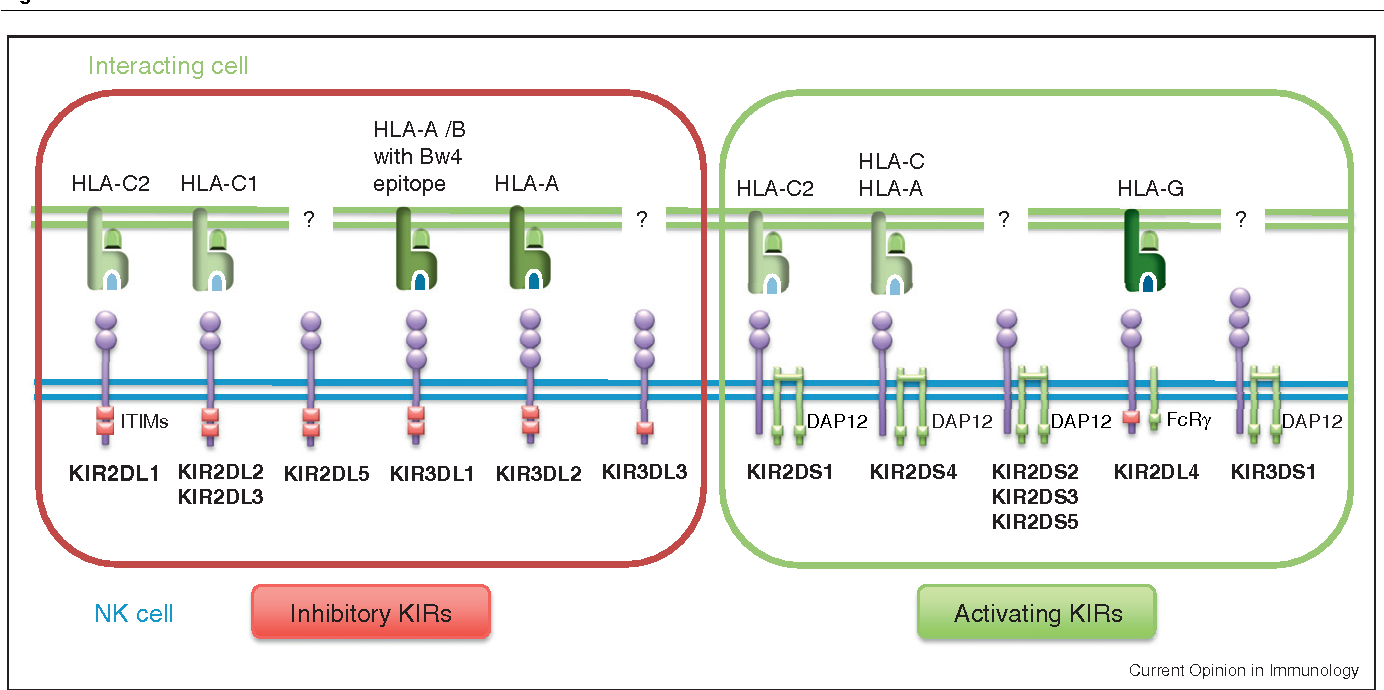
\includegraphics[width=\textwidth]{./img/KIR_nomenklatura2.png}
		\caption{KIR geny a jejich vazebné ligandy. Pokud je v obrázku ? značí to, že pro daný receptor neni znám vazebný ligand. \cite{KIR_img_nomenklatura}}
		\label{fig:img_kir_ligand}
\end{figure}

\noindent
NK buňky ustavičně prohledávají své okolí a testují přítomnost příslušných HLA ligand pro své KIR receptory. Pokud je příslušný HLA ligand přítomen naváže se na NK buňku (\ref{fig:kir_princip} případ~1). Tímto systémem jsou ochráněny vlastní buňky. Pokud přítomen není je spuštěna cytotoxická reakce a zkoumaná buňka je zníčena.
\\
\\
Některé virem napadené buňky potlačují propsání HLA ligand na povrch buňky a tím se brání cytotoxicitě proti T lymfocitům, ale naopak jsou více citlivější na cytotoxicitu proti NK buňkám, jak je zobrazeno na obrázku \ref{fig:kir_princip} případ~3.
\begin{figure}[H]		
		\centering
		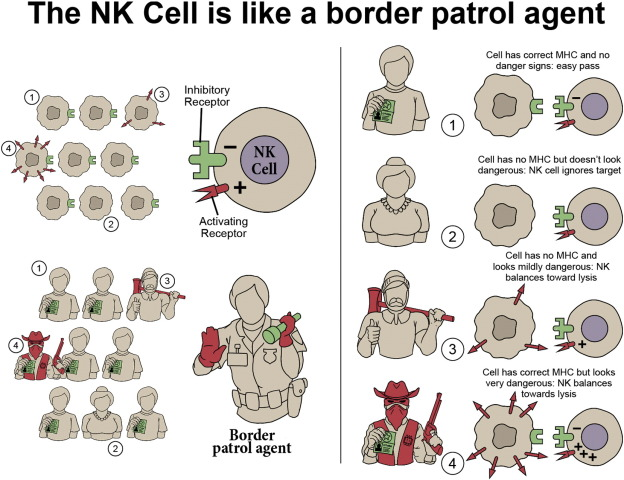
\includegraphics[width=\textwidth]{./img/NK_princip.jpg}
		\caption{Přirovnání fungování natural killer buňky k pasové kontrole. V pravé části jsou zobrazené případy které mohou nastat když natural killer buňka potká jinou buňku. V prvním případě je tělu vlastní zdravá buňka, kde se KIR receptor naváže na HLA ligand a k cytotoxitické reakci nedojde. Druhým případem je červená krvinka. K reakci NK buňky opět nedojde, protože na zkoumané buňce nepřevažují aktivační receptory. V 3 případě je to nádorová buňka, která schová HLA ligand (může nastat po transplantaci kostní dřeně) a tím se "schová" proti T- lymfocytům. Avšak aktivační receptory převládají a tak k cytotoxicitě dojde. Ve 4 příkladě je nádorová buňka nebo virem nakažená buňka (stresové ligandy). Aktivační receptory převládají k cytotoxicitě dojde.\cite{KIR_img_princip}}
		\label{fig:kir_princip}
\end{figure}



\subsubsection{KIR haplotyp}
KIR haplotyp je vyjádření jaké konkrétní KIR geny genom obsahuje. Doposud nebylo zavedeno konkrétní pravidlo na jejich pojmenovávání. Avšak bylo navrženo, aby každý KIR haplotyp byl označen $"KH-"$ následovaným trojmístným číslem, které bude označovat konkrétní haplotyp. Bylo by tak možné pojmenovat 999 haplotypů. \cite{imgt_hla_database}
\\
\\
Dále by se haplotypy rozdělovali na dvě skupiny A a B. Skupina B musí obsahovat alespoň jeden z genů KIR2DL5, KIR2DS1, KIR2DS2, KIR2DS3, KIR2DS5 a KIR3DS1. Naopak skupina A neobsahuje ani jeden z těchto genů. Z tohoto pravidla je patrné, že haplotypy B mají vždy více aktivačních KIR než haplotypy A. Za trojmístným číslem by tedy dále bylo písmeno A nebo B.
\\
\\
Nakonec by byl připojen 17-ti místný binární kód, který by označoval přítomnost $"1"$ či absenci $"0"$ genu. Pořadí genů by odpovídalo pořadí v genomu od centrometrické části k telemetrické části.
\\
\\
Výsledné pojmenování by mohlo vypadat následovně:
\begin{align}
   \label{kir_haplotyp} KH-001A-11100010011011011
\end{align}

\noindent
Je třeba si zde uvědomit, že každý jedinec má 2 KIR haplotypy. Je tedy možné dostat 4 kombinace - A/A, A/B, B/A nebo B/B. Haplotyp jedince je označován za A v případě kdy má kombinaci A/A a za B v případě jedné z kombinací A/B, B/A nebo B/B. Je možné si povšimnout, že u haplotypu B převládají inhibiční KIR geny a proto jsou dárci lépe přijímáni.
 
\begin{figure}[H]		
		\centering
		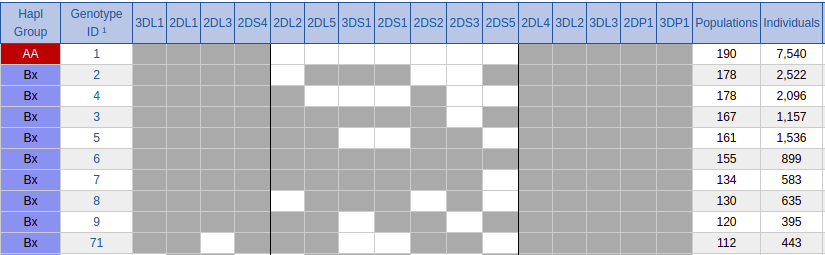
\includegraphics[width=\textwidth]{./img/KIR_haplotypy_priklad.png}
		\caption{Deset nejčastější KIR haplotypů. Šedý obdelník značí přítomnost genu, bílí jeho nepřítomnost. \cite{kir_genotypes_10}}
		\label{fig:kir_haplotypy_10}
\end{figure}

\noindent
Na základě variací obsahu genů by bylo možné vytvořit nepřeberné množství KIR genotypů. Na základě sesbíraných haplotypů byl sestaven model, který toto množství mírně redukuje. Haplotyp se rozděluje na dvě části na centrometickou a telometrickou. Kdy jednotlivé části mezi sebou mohou být kombinovány. Existují vzácné varianty, které se do tohoto modelu nehodí. \cite{KIR_haplotypy_ct}
\begin{figure}[H]		
		\centering
		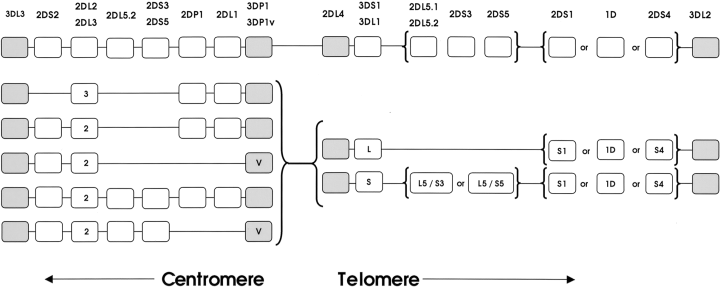
\includegraphics[width=\textwidth]{./img/KIR_haplotypy.png}
		\caption{Rozdělení KIR genů na centrometrickou a telometrickou část, pojmenování je na základě, zda je úsek blíže k centromeru nebo k telomeru (viz obrázek \ref{fig:chrmosome}). \cite{KIR_haplotypy_ct}}
		\label{fig:kir_aplotypy_ct}
\end{figure}

\noindent 
\textbf{Centrometická} polovina je charakterizována přítomností jednoho z 2DL3 nebo 2DL2, vzácně nemusí být přítomný ani jeden. V případě 2DL2 je následně přítomen 2DS2. Tento pár genů se následně objevu v kombinaci s -2DP1, -2DL1 a -3DP1. 2DL5 gen je v centromerické části párován s 2DL2 a 2DS3, ve vzácných případech se může objevit i s 2DL2 a 2DS5. Oproti tomu při přítomnosti KIR2DL3 se dále vyskytuje KIR2DP1, -2DL1 a -3DLP1.
\\
\\
\textbf{Telometrická} polovina haplotypu je charakterizována přítomností jednoho z 3DL1 nebo 3DS1, vzácně nemusí být přítomný ani jeden. Gen 3DL1 se následně objevuje v přítomnosti s 2DS4, 1D nebo 3DL2. V případě KIR3DL se jedná o takzvaný krátký segment obsahující 2DS4 nebo KIR1D zakončené 3DL2. V případě KIR3DS1 se jedná o dlouhý segment obsahující 2DL5, párovaný s 2DS3 nebo 2DS5, následovaný 2DS1, 2DS4 nebo KIR1D opět zakončený 3DL2. \cite{KIR_haplotypy_ct}
\\
\\
Podle některých studii zabývající se vlivem KIR haplotypů na výsledky transplantace bylo zjištěno, že KIR haplotypy ovlivňují výsledky u akutní myeloidní leukémie. Ve srovnání s haplotypem A měl haplotyp B, především jeho centrometická část, ochraný účinek před návratem nemoci a zárověň zvýšil pravděpodobnost přežití pacienta. Na základě této skutečnosti se mohou dárci řadit do tří skupin best, better a neutral. Best je definován jako Cen-B/B a Tel-x/x, better jako Cen-A/x a Tel-B/x, a neutral v případě jedné B části nebo žádné. \cite{KIR_haplotypy}
\\
\\
TODO tohle je divný vždyť jedna ta část B je i u better?
\\
\\
Dále je možné se setka s takzvaným B-skóre



TODO podle tohohle se právě určuje B-content score pro definování úrovně B haplotypu, best varianta pro transplantaci je B/B (cen) s B/B (tel), viz další komentář


We defined the KIR B–content score for each donor's KIR genotype as the number of centromeric and telomeric gene-content motifs containing B haplotype–defining genes. Permissible values for the KIR B–content score are 0, 1, 2, 3, and 4 (Figure 1C). A calculator for classification of the donor KIR B status (best, better, neutral) may be found at http://www.ebi.ac.uk/ipd/kir/.
\\
\\
TODO to znamená že to b score je to best, better, neutral a ještě tam je přidaný none of this? 


\section{Nalezení vhodného dárce}
Mezi rizika při transplantaci krvetvorných buněk patří reakce štěpu proti hostiteli nebo relaps oněmocnění (návrat nemoci). Ač je dárce vybírán podle shody v HLA znacích, sekundární kriteria jako jsou pohlaví a věk hrají také roli pro úspěšnost transplantace. Navíc podle nedávných studiích výsledky příjetí štěpu ovlivňují nejenom HLA geny ale i non-HLA geny. Jedním z nich může být právě killer immunoglobulin-like receptor (KIR). V případě kdy by bylo nalezeno více vhodných dárců, tj. se shodou 10/10 nebo 9/10, vybíralo by se následně podle KIR genů. \cite{KIR_transplantace_jindra} \cite{Frycova_bakalarka}
\\
\\
Při určování shody dárce a pacienta se rozhoduje na základě schody alel u genů HLA -A, -B, -C, -DRB1, -DQB1. Díky velké diverzitě HLA genů je počet možných kombinací několik miliard. Některé kombinace genů se vyskytují na základě oblasti či národnosti častěji nebo mohou být naopak vzácné. HLA geny se obvykle dědí jako blok (cely haplotyp), avšak ve výjmečných případech může dojít k rekombinaci. Z tohoto důvodu je nejsnadnější nalést shodu v pokrevním příbuzenstvu.
\\
\\
Jelikož každý jedinec má dvakrát geny na pozicích HLA -A, -B, -C, -DRB1 a -DQB1 (jednu pětici od otce, druhou pětici od matky), je maximální shoda 10/10 (shoda obou alel v lokusech). Čím je shoda menší tím větší je riziko nepřijetí stěpu. U nepříbuzných jedinců lze tolerovat shodu 9/10 či 8/10. \cite{Frycova_bakalarka} \cite{KIR_transplantace_jindra}
\\
\\
V posledních letech se objevuje Haploidentická transplantace, kdy je možné použít krvetvorné buňky příbuzného se shodou pouze jednoho haplotypu (5/10) například všichni rodiče a děti. Umožnuje to podávání chemoterapie pár dní po transplantaci, která zníčí všechny buňky, které tělo nepřijme. Využívá se toho hlavně v případech časové tísně, kdy není čas hledat dárce v registrech. \cite{haploidenticka_transplantace}
\\
\\
KIR geny se stejně jako HLA dědí celý blok. Jelikož HLA se nachází na 6 chromozomu a KIR na 19, tak shodní dárci v HLA znacích se jen menšinově shodují v KIR genech. V případě příbuzného dárce shodujícího se v HLA znacích je pouze 25\% shodných také v KIR. \cite{KIR_haplotypy}
\\
\\
TODO možná informaci o B-content score za tohle, proč u více shodných se řeší KIR, že se vybírají B haplotypový dárci a že v poslední době se řeší, zda kromě haplotypu nemají vliv konkrétní alelické varianty KIR genů (to je to, proč vy to žešíte v diplomce)
\\
\\
K zjištění konkrétních alelických variant se pro tzv. typizaci využívají sekvenační metody, typicky s polymerázovou řetězovou reakcí. 


\section{Bordel haplotypy}

TODO budu to tam dopisovat? KIR2DL5 (Where two or more genes have very similar structures and have very similar sequences, they may be given the same number but distinguished by a final letter: for example, the KIR2DL5A and KIR2DL5B genes. The similarity of these two genes suggests they are related by a recent gene duplication event. ),




\chapter{Sekvenační metody získávání DNA dat}
Po pojmem sekvence DNA se skrývá posloupnost písmen představujících primární strukturu reálné nebo hypotetické molekuly čí vlákna DNA, které nese nějakou informaci. Jednotlivá písmena jsou označována jako nukleotidy nebo nukleové báze. Nukleové báze mohou být A~-~adenin, C~-~cytosin, G~-~guanin a T - thymin. \cite{genome_gov}
\\
\\
\noindent
Příkladem může být následující úsek sekvence na základě obrázku \ref{fig:chrmosome} 
\begin{align}
   \label{sekvence_prikad} ACGTCA
\end{align}

\noindent
\textbf{Sekvenování DNA}, někdy pouze sekvenování, jsou biochemické metody, kterými se zjišťuje pořadí nukleotidů (A, C, G, T) v sekvenci DNA. Díky tomu je možné zjistit typizaci konkrétního člověka. Sekvenační metody se liší zejména délkou řetězce, kterou dokáží zpracovat, cenou a rychlostí sekvenace. Pro porovnání sekvenování celého genomu Sangerovo metodou by stálo několik milion dolarů a trvalo zrhuba 10 let. Při použítí dnešních metod by cena byla zhruba tisíc dolarů. Většina sekvenačních metod využívá vlasnosti přitahováním báze do páru pouze jednou konkrétní bází. To znamená že se adenin vždy páruje s thyminem a cytosin se vždy páruje s guaninem. Z těchto párů vzniká již známá dvojitá šroubovice DNA. Při sekvenování je možná se často setkat, že se sekvenuje jen kónkrétní kus DNA, který je zrovna potřeba. Největším problémem u sekvenování je, že ready vzniklé ze sekvenátoru jsou jen kousky, které je třeba poskládat zpět. K tomu slouží zarovnávání. \cite{sekvenovani_ziva}
\\
\\
TODO možná tady ještě napsat něco o přípravě na sekvenování - je to dyžtak v tý přednášce co nám řikala na FAV
\section{Sanger sequencing}
Sanger sekvenování využívá možnosti namnožení řetězce díky vzájemnému přitahování konkrétních bází. V prvním kroce replikace jsou nastříhané řetězce rozděleny na dvě vlákna. Lze si představit, že tyto dvě oddělená vlákna jsou dána do směsy, kde plavou jednotlivé nukleotydy spolu s upravenými nukletidy, které nesou specifickou fluorescenční barvu a za které neni možné nic navázat. Následně za pomoci střídaní teploty volně plující nukleotidy tvoří postupné páry s řetězcem, který chceme namnožit. Pokud se povede celý řetězec namnožit je odtržen a může se dále množit. Postupně ale bude docházet k navazováním nukleotidů s fluorescenční barvou. Tím se vytvoří nekolik různě dlouhých sekvencí zakončených označeným nukleotidem. Podle jeho barvy je možné poznat o jaký nukleotid se jedná. Následně jsou za pomoci elektorforézy seřazeny v gelu podle délky. Elektroforéza rozděluje různě dlouhé sekvence na základně odlišnosti pohybu v elektrickém poly. Kratší doputují dále než delší. Pomocí sanger metody je možné sekvenovat řetěce dlouhé až 1000 bází.   

\begin{figure}[H]		
		\centering
		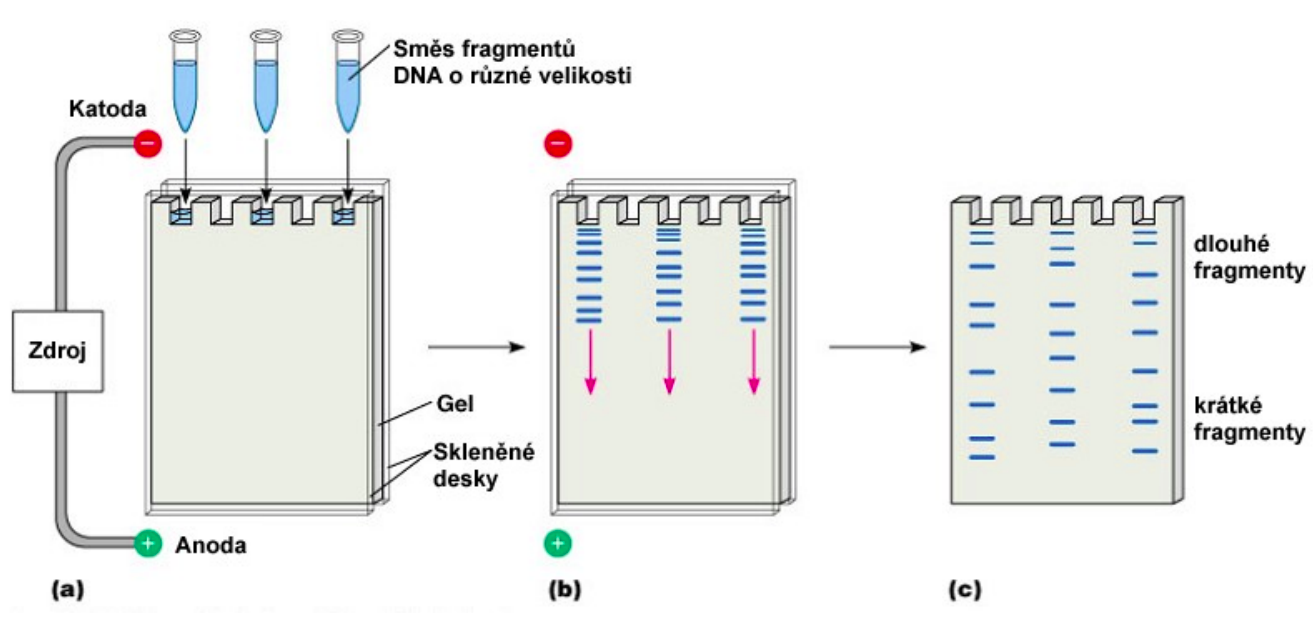
\includegraphics[width=\textwidth]{./img/elektroforeza.png}
		\caption{Elektroforéza. \cite{elektroforeza_img}}
		\label{fig:elektroforeza}
\end{figure}
 
\section{NGS next-generation sekvenování}
Next-generation sekvenování někdy označováno jako metody druhé generace jsou v porovnání se Sangerovo sekvenováním rychlejší a levnější, na druhou stranu ale dokáží zpracovávat jen řetězce dlouhé 100 až 500 bází, mají menší přesnost a časteji chybují. Jejich rychlost spočívá především ve schopnosti detekovat přidávání bází jednu po druhé a zároveň sekvenovat tisíce až miliony rozdílných molekul DNA najednou. 
\\
\\
Všechny tyto metody si předpřipraví řetězce nastříháním na krátké části a připevenín takzvaného adeptéru na jejich konec. Adaptér je krátká molekula DNA, která slouží k uchycení sekvenovaného úseku na pevný povrch. Řetězce DNA jsou namnoženy díky čemuž vzniknout klastry identických molekul koncentrovaných v jednom místě. Díky tomu je posílen signál, který by z pouhé jedné molekuly nebyl dostatečně silný. Tento signál je zachycen kamerou. Jeden z důvodů popularity NGS metod jsou i cenově dostupné stolní sekvenátory.
 

\subsection{454 sekvenování a Ion Torrent}
Pomocí 454 sekvenování je možné analyzovat více než milion molekul DNA najednou a délka každé jednotlivé sekvence se pohybuje okolo 700 až 1000 bází. V prvním kroku sekvenování je fragment DNA přichycena na malou "kuličku" na jejimž povrchu se postupně namnoží až kuličku zcela pokryjí identické fragmenty DNA. Následuje vložení kuličky i s DNA do jedné z milionů komůrek na destičce s reakční směsí. Postup znázorněn na obrázku \ref{fig:sekvenovani_454}. V určitém momentě je do této směsy přidán vždy jen jeden typ báze. Mezi jednotlivými fázemi přidávání určité báze jsou přebytečné nukleotidy z předešlého kroku odstraněny. To znamená že v reakční směsy je vždy jen jeden typ nukleotidů. Během vložení každé nové báze do rostoucího řetězce DNA je uvolněna molekula zvaná pyrofosfát, která spustí několik chemických reakcí. V poslední fází enzym luciferáza vydá světelný záblesk, který je možné zachytit citlivou kamerou.  Tento postup se nazývá pyrosekvenování. V případě, kdy je do řetězce přidáno několik stejných bází za sebou, například gen obsahuje podřetězec AAA, je vyzářeno, v našem případě, třikrát více světla než v případě jedné přiřazené báze. Kamera snímá celou destičku a na základě. která komůrka se rozsvítí pozná, kde proběhlo přidání báze. Intenzita světla pak určuje kolik bází bylo přidáno na jednou. 


\begin{figure}[H]		
		\centering
		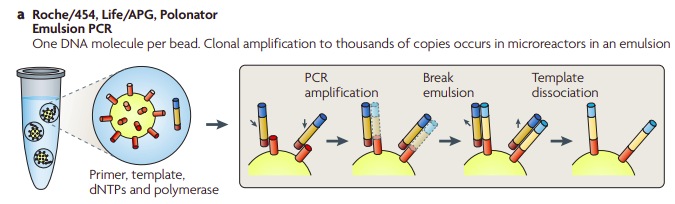
\includegraphics[width=300px]{./img/sekvenace_454_1.png}
		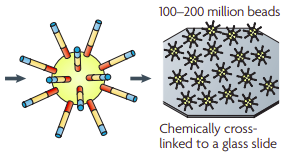
\includegraphics[width=150px]{./img/sekvenace_454_2.png}
		\caption{454 sekvenování. \cite{ngs_merzker}}
		\label{fig:sekvenovani_454}
\end{figure}

\noindent
Sekvenování Ion Torrent funguje na podobné princupu sekvenování s rozdílem, že místo světla se měří změna pH v reakční směsy. Podle intenzity změny pH lze pak poznat kolik nukleotidů bylo přidáno do rostoucího řetězce.
\\
\\
Hlavní slabinou těchto dvou metod je značná chybovost při přidání mnoha stejných nukleotidů do řetězce za sebou. Například pří přidání 10 A, nebude odpověď jednoznačná zda je to 10 A nebo 9.


\subsection{Illumina}
Při sekvenování pomocí Illumina jsou páry dvoušrobovice rozděleny na dva řetězce. Jednotlivé řetezce jsou následně přichyceny na malou destičku pomocí adaptéru. Každý řetězec se následně opakovaně množí až na destičce vznikne několik shluků. Přidání jedné molekuly ke druhé probíhá obdobně jako u Sanger sekvenování. Každý shluk tvoří jednu skupinu vzájemně identických řetězců. Mezi volné nukleotidy jsou opět zahrnuty nukleotidy označeny fluorescenční barvou za které nelze nic navázat. Oproti sangerovu sekvenování je ale tato blokace vratná a po přečtení citlivou kamerou dojde k odstranění blokující části molekuly. Počítač si pak následně zpětně spočítá co to bylo za barvu (nukleotid). \cite{illumina} \cite{sekvenovani_ziva} 


\subsection{SOLiD}
SOLiD (Sequencing by Oligonucleotide Ligation and Detection) se spoléhá na enzym ligáza. Enzym je bílkovina, která určuje rychlost chemických reakcí. Enzym ligáza konkrétně umožňuje připojení jednořetězcových molekul k stávajícím řetězcům. K teplátu jsou přidávány takzvané sondy, což jsou kousky DNA. Sondy začínají všemi možnými dvojkombinacemi čtyř základních nukleotidů. V součtu je 16 sond. Na každé sondě je jedna ze čtyř flurescenčních barev. V jednotlivých krocích jsou sondy připojeny k rostoucímu řetězci. Následně je přečtena fluorescenční barva, která je odstraněna a může se tak navázat další sonda. Z výsledného signálu lze pak odvodit sekvenci DNA.


\section{Metody třetí generace}
Velkým rozdílem oproti druhé generaci je že DNA templát není před sekvenování namnožen a je čten pouze z jedné původní molekuly. Existuje například PacBio od Pacific Bioscience, který k detekci využívá fluorescenčně značené nukleotidy. Díky jeho vysoké citlovosti je možné v reálnám čase zachytit přidání i jediného nukleotidu do jediného řetězce DNA. Další zástupce je Oxford Nanapore jehož výhodou je jeho velikost. Oxford využívá odlišného tvaru bází. Obě metody jsou schopné přečíst přes 10 tisíc bází v rámci jedné analyzované molekuly DNA. 


\section{Read}
Read je sekvence bází odpovídající celému genomu či nějaké jeho části. Ready jsou typický výstup sekvenačních technik, kdy výstupem je sekvence nukleotidů o kterých nikdo neví co znamenají. Může to být gen, část genu nebo několik různých genů. Význam readu (o jaký gen se jedná) se zjišťuje zarovnáváním, kdy se daná sekvence porovnává vůči referenčnímu genu.
\\
\\
TODO je to z wiki, musím tady nutně udávat zdroj?   
\section{Single-end, paired-end a mate-pair}
Single-end je sekvenování pouze jednoho konce molekuly. Nevýhoda tohoto způsobu se projeví především na krátkých readech, kde se zvýší problém jejich správného umístění. Oproti tomu v případě paired-end se sekvenuje z obou konci daného úseku. Vzniklé dva ready jsou označeny a zárověň je známá jejich vzdálenost mezi oběma ready, která se pohybuje od 200 do 400 bp (base pair). V případě ART to naznačuje stejný název souboru spolu s 1 čí 2 na jeho konci. Mate-pair je v podstatě paired-end s rozdílem, že je mezi ready větší vzdálenosti od 2 do 5 kb (kilobase) - takže přibližně 2000 - 5000 bp. \cite{illumina}  
\\
\\
TODO obrázek je z trochu blbího zdroje nejsem si jistá jestli ho můžu použít, ale mě přišel dobrej. \url{https://www.yourgenome.org/facts/how-do-you-put-a-genome-back-together-after-sequencing}
\begin{figure}[H]		
		\centering
		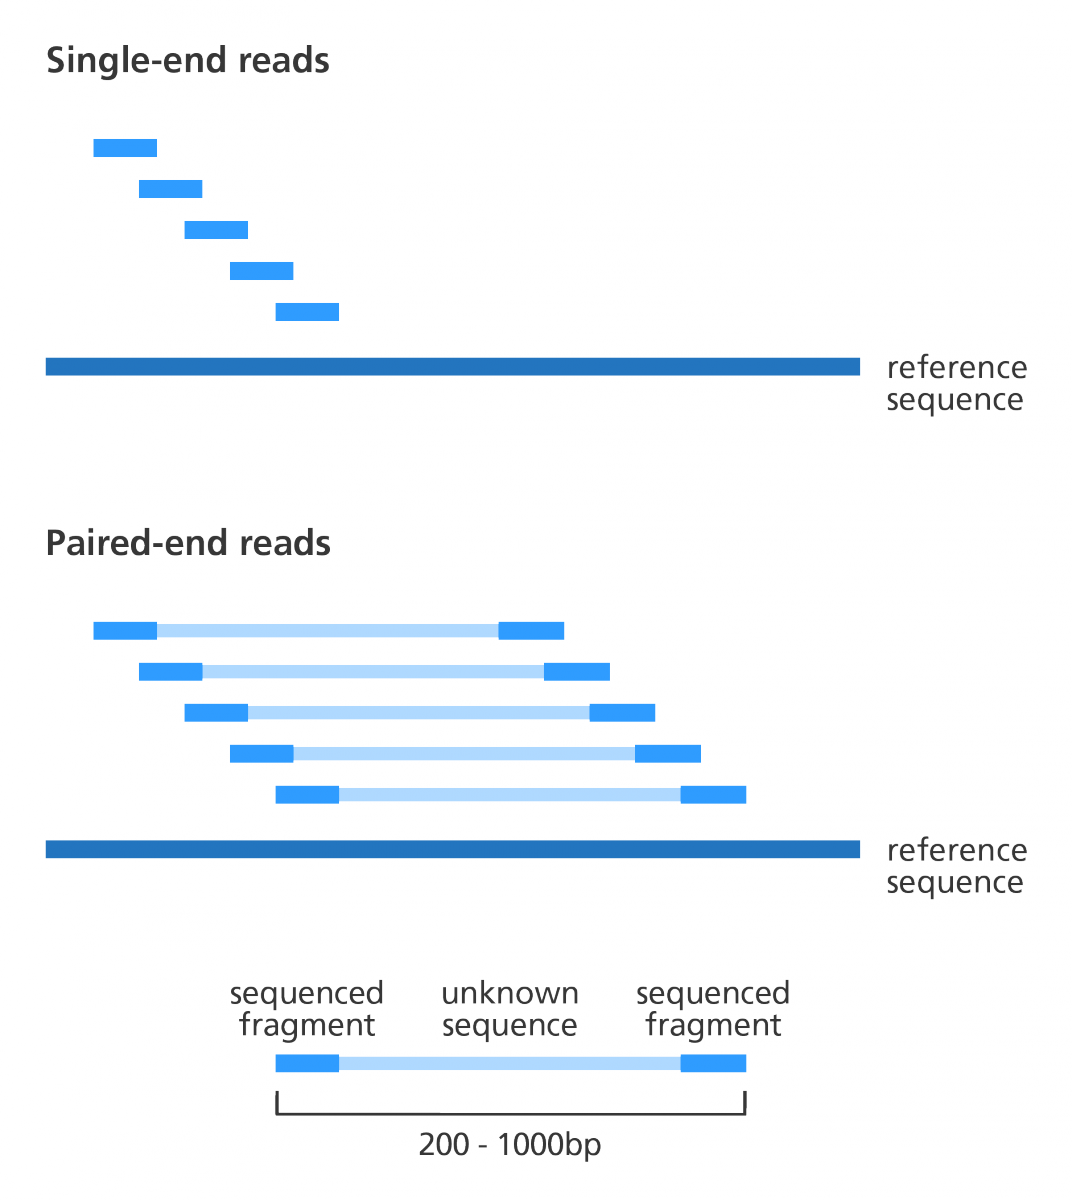
\includegraphics[width=200px]{./img/single_end_pair_end_reads_yourgenome.png}
		\caption{Single-end a paired-end read.}
		\label{fig:single_end_paired_end}
\end{figure}

\section{Bordel}
Sekvenování mRNA s použitıím NGS technologií umožňuje měření genové exprese celého
transkriptomu. Postup a provedení RNA-seq experimentu je znázorněn na obr. 14.
Prvním úkolem je vyčistit zkoumaný vzorek o rRNA, tRNA a mitochondriální RNA,
které u prokaryot i eukaryot tvoří přibližně 75 procent všech RNA molekul. Navzdory použití
purifikačních metod, mezi které patří například poly(A)purifikace a DNS normalizace,
sekvenační data mohou obsahovat menší množství těchto RNA molekul [59]. Ty mo-
hou být odfiltrovány v následujícíh krocích bioinformatickými postupy. Zbylá mRNA
je poté nastříhána na menší části, a je z ní připravena knihovna krátkých fragmentů s
navázanými adaptory. Ty jsou poté sekvenovány sekvenačním přístrojem a jako výsledek
získáme tzv. ready.
Samotné ready však nemají žádnou vypovídající hodnotu, a proto jsou dále bioinformat-
icky zpracovány. Namapováním na referenční sekvenci zjistíme jejich genomickou pozici,
ze které byly odvozeny. Většina readů je namapována na exony, což jsou transkripčně
aktivní jednotky, a pouze malé množství readů je namapováno na transposony. Ready
které nejde namapovat v celku, jsou rozděleny na menší části a ty jsou namapovávány
zvlášť. Rozdělené ready umožňují jednodušší identifikaci mezer mezi exony (angl. splice
junctions)
tohle je z tý diplomky single-pair

\chapter{Analyza dostupných bioinformatických nástrojů pro zpracování NGS dat}

\section{ART}
ART (next-generation sequencing read simulator) je sada simulačních nástrojů, které generují syntetické ready, jako kdyby byli získány sekvenováním pomocí NGS. Nástroj ART dokáže simulovat single-end a paired-end ready ze sekvenátorů Illuminas, 454 společnosti Roch a SOLid od společnosti Applied biosystém. Ready, vytvořené nástrojem ART jsou používány pro testování a analýzů nástrojů zpracovávající právě NGS sekvence jako například zarovávání (nástroj Bowtie). Při použítí nástroje ART je vstupním souborem sekvence genů na základě kterých jsou vygenerovány ready. \cite{art}
\\
\\
Podle \cite{art} je dostupných několik simulačních nástrojů (Wgsim, MetaSim, SimSeq, FlowSim), které fungují dobře pro sekvenátory pro které byli určeny, ale žádný z nich se nedokázal vypořádat se všemi nejvíce používanými. Jejich slabinou je především v generovaní chyb na základě jednotlivých módů konkrétního sekvenátoru. Nejčastější chyby jsou substituční a vložení čí smazání (INDEL - insert-deletion). ART obsahuje technologické profily chyb a navíc mu může použít i uživatelský profil chyb. Profily které obsahují délky readů a chyby byly získány z datasetu skutečných sekvenovaných dat. 
\\
\\
TODO možná napsat co znamenají konkrétní chyby
\\
\\
TODO
Proč? No protože přesně ví co tam dávají za data, protože mu podšoupnou ten referenční genom a tak pak můžou dobře sledovat co ten zarovnávač s tím dělá. 
A proč je to o tolik výhodnější než když by měli nějakej realnej dataset? 
Možná že si tam můžou ty chyby navolit tak jak se jim hodí?
Jako bude v tom míň chyb, ale stejně. 
\\
\\
\textbf{Illumina} je sekvenování založené na vratném umístění báze označené barvou do rostoucího řetězce jehož nejčastější chybou je substituce. Pravděpodobnost chyby substituce je určená na základě kvality skoré dané báze, které je závislé na pozici v rostoucím řetězci. Průměrné kvality skore klesá v závislosti na zvyšování pozice báze. ART simuluje substituční chybu na základě tohoto skore a emprického modelu získaného z trénovacích datasetů. INDEL chyba je simulována jen na základě empirického rozdělení z trénovacích dat. Pro paired-end simulaci, ART využívá dvou rozdílných kvality skore pro každý pár readu jiný. 
\\
\\
\textbf{454} je sekvenování při kterém se zachycuje vyzářené světlo na základě toho pokud se báze přidala do řetězce či nikoliv. Jeho dominantní chybou je tedy nesprávné určení počtů přidaných bází. Pravděpodobnost chyby roste s frekvencí dlouhých úseků obsahující stejnou bázi. Proto ART modeluje rozdělení chyb na základě délky úseku obsahující stejnou bázi spolu s Markovovy řetězci.
\\
\\
\textbf{SOLid} je založené na označení čtyř barev pro 16 různých skupin bází. Pro paired-end read simulaci délky fragmentu je použito Gausovské rozdělení. Rozdělení chyb je založena na empirické znalosti získané z readů generovaných Applied Biosystémem. ART zároveň nabází nastavené chybovosti základě lineárního měřítka. 
\\
\\
ART je implementován v jazyce C++ a je dostupný s licencí GPL verze~3 pro operační systémy Linux, MacOs a Windows. Je možné ho použít i jako C++ package. Pro jeho spuštění je nutní mít nainstalovaný compilator GNU g++ 4.0 nebo vyšší a knihovnu GNU gsl. 
\\
\\
Data získána z FN Plzeň byla sekvenována nástrojem Illuminas proto i syntetické ready budou simulovat tento sekvenátor.   Výstupy se čtou ve formátu FASTQ a zarovnání ve formátu ALN. může generovat zarovánávání také ve formátu SAM nebo UCS BED. 


\section{Bowtie}
Bowtie je rychlý a paměťové efektivní nástroj pro zarovnávání krátkých sekvencí DNA na velké genomy. Bowtie2 je schopný zarovnat více než 25 milionů readů dlouhých 35 bp za hodinu (při běhu na jednom CPU) pro lidský genom s malým využím paměti. Bowtie využívá FM indexaci s Burrows-Wheeler transformací (BWT) a přidává k ní backtracking pro sledování nekonzistence. Novější verze Bowtie2 by měla by oproti Bowtie1 citlivější a rychlejší na delší ready než je 50 nukleotidů a navíc je oproti první verzi schopná se vypořádat z chybami vložení čí smazání báze způsobené sekvenováním. Na lidský genom potřebuje Bowtie2 3.2 gigabajtů RAM. Nástroj bowtie je implementovaný v jazyce C++ s použitím knihovny SeqAn a je open source. Podporuje standardní vstupní formáty FASTQ a FASTA.  Výstupní zárovnání z Bowtie je ve formátu SAM, což umožňuje návaznost s dalšími nástroji jako je třeba SAMtools. \cite{bowtie} \cite{bowtie2}   
\\
\\
Zarovnávání bývá prvním krokem v mnoho genomických pipelinách. Často je to jejich nejpomalejší část, protože pro každý read musí zarovnávač vyřešit obtížný výpočetní problém. Určit pravděpodobné umístění v referenčním genomu. Mnoho zarovnávačů používá indexy k rychlému snižování kandidátů pro umístění zarovnáváného readu. Bowtie vytváří indexy referenčních genů permanentní a lze je tak použít napříč běhy. Algoritmus FM indexu obyvykle funguje na vyhledává přesně shody. V případě hledání umístění readů na referenční gen není toto řešení použitelné, protože ready mohou obsahovat chyby vzniklé sekvenováním případně genové mutace. Proto bowtie každé zarovnání zakládá na kvalitě znaku báze v daném readu. Bowtie postupně vytváří dlouhý sufix. Pokud se sufix nevyskytuje v textu pak se může algoritmus vrátit a v již vytvořeném sufixu nahradit bázi za jinou. Dále pokračuje obdobným způsobem. Pokud by měl algoritmus na výběr substituovat za více bází vybere tu s nejnižší kvalitou znaku v readu. Protože bowtie algoritmus v základu bere první přijetelné řešení je možné, že jeho nalezené řešení není to nejlepší. Pro nalezení toho nejlepšího řešení je třeba použít přepínač $--best$, jeho funkčnost je ale na úkor rychlosti, která může být 2x čí 3x pomalejší. Zároveň je možné nastavit maximální počet nahrazených bází v readu. \cite{bowtie}
\\
\\
V případě že backtracking mechanismus není uspěšný může docházet k jeho nadměrnému vyskytu. Bowtie se tento jev snaží zmírnit dvojím indexováním. První index obsahuje BWT genomu a je označován jako dopředný index. Druhý obsahuje opět BWT genomu, ale se znaky v sekvenci v opačném pořadí, označovaný jako zrcadlový index. Read je pak v půlce rozdělen na dvě části a jejich zarovnávání probíhá odděleně tak, že je vždy backtracking povolen jen v dané části, která je zrovna zarovnávána. Pravá část je zarovnáváná podle dopředného indexu a levá část je zarovnávána podle zrcadlového indexu. 
\\
\\
TODO já nevím mě občas přijde že opisuju ten článek, a nevím jestli je to dobrý a stejně tomu na půl nerozumím .. 
\\
\\
TODO tohle prostě nedává smysl..možná se mrkni ještě na stránky bowtie jestli tam o tom něco neni napsaný
\\
\\
Ačkoliv je full text minute index často použávanej kvůli své rychlosti a nízké paměťové náročnosti ale neni vhodný na dlouhé zarovnávání které může obsahovat mezery. Bowtie 2 combinuje obojí sílu full text minute index s flexibilitou a 

Zarovnávači používají indexy k rychlému snižování kanditádů 
aligmenty mají maximální počet kolik změn tam může být 
S mezerami se nám prostor pro vyhledání správné pozice ještě zvětší
ale tento prostor může být změnšen díky dvojímu indexování bezmezerových aligmentů
Zarovnávání pomocí indexů, ale může být neefektivní v případě pokud zarovnávaný read obsahuje mezery
 
 mezery zvětšují prohledávaná prostor a redukují efektivitu prořezávání
 
  

Alignment gaps can result either from sequencing errors or from true insertions and deletions. 
TODO co je sakra true insertions and deletions - jako genová mutace? 

Bowtie 2 rozšiřuje full-text minute index aby bylo možné se vypořádat s mezerami.
a rozděluje algoritmus zarovnání na dvě části
-bezmezerový vyhledávání seed - semene? , který vyhledává na základě full text minute indexu
- a mezerové které využívá dynamckého programování a těží z efektivity single- instruction multiple data parrall processing
 SIMD mě navádí na vektory? To má být to zrychlení? Jen že ten prostor dokáže rychlejc projít?
\\
\\
Pro každý read
\begin{enumerate}
	\item extrahování seed z readů a jeho zpětné doplňky - ne to je to dvojí indexování
	\item extrahované podřetězce jsou zarovnány na referenci v bezmezerové modelu za pomocí full-text minute index
	\item seed aligmenty jsou priorizovány a jejich pozice na referenčním genom jsou spočítány z Full text minute indexu
	\item seedy jsou rozšířeny do úplného zarování pro zvýšení výkonu je použito SIMD -accelerated dynamic programming.
\end{enumerate}

TODO možná dopsat že díky experimentu 1 a 2 a pak porovnání výsledků když jsem to pustila blbě na všechny ty geny a pak když jsem to pustila na jeden jsem vydedukovala jak to bowtie zarovnává nebo bych to měla dát až k tomu experimentu přímo? 

\subsection{Burrows-Wheeler transformace}
Burrows-Wheelerova transformace (BWT) je reverzibilní permutace řetězců v textu. Původně byla používána pro kompresy dat. Indexace založená na BWT umožňuje efektivní vyhledávání ve velké textu s malou paměťovou náročností. 
\\
\\
BW transformace řetězce T, $BWT(T)$, je zobrazena na obrázku \ref{fig:bw_transform_1}. Znak~\$ je připojen na konec řetězce a zároveň musí platit, že se tento znak se v řetězci nevyskytuje. Burrows-Wheeler matice řetězce T je konstruovaná jako všechny cyklické rotace řetězce T, které byli seřazeny podle abecedy, kde znak \$ se bere, že je na záčátku abecedy. Výstup, BWT(T) pak představuje poslední sloupec matice. Tento řetězec má stejnou délku jako původní řetězec T. \cite{bowtie} 

\begin{figure}[H]		
		\centering
		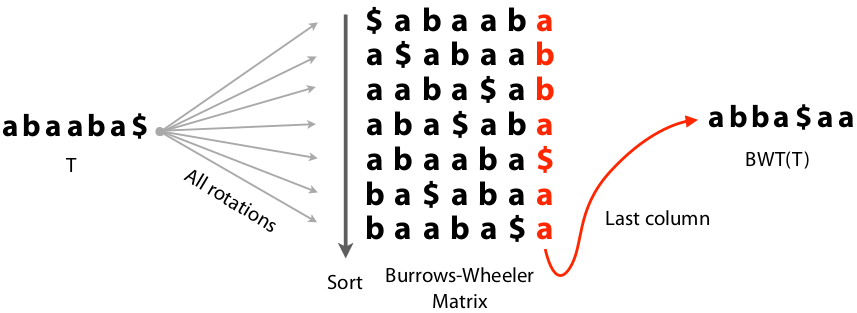
\includegraphics[width=.8\textwidth]{./img/BWT_1.png}
		\caption{Burrows-Wheeler transformace řetězce T. \cite{bw_transform}}
		\label{fig:bw_transform_1}
\end{figure}

\noindent
Burrows-Wheeler matice má vlastnost, která se nazývá last first mapping (LF). To znamená, že i-tý výskyt znaku X v prvním sloupci je i-tý výskyt znaku X v posledním sloupci. V případě přidání indexu do řetězce T je toto pravidlo pro znak $a$ zobrazeno na obrázku \ref{fig:bw_transform_lf}. Obdobně to platí i pro ostatní znaky v řetězci.

\begin{align}
   \label{rerezec_t} T - a_0 \: b_0 \: a_1 \: a_2 \: b_1 \: a_3 \: \$
\end{align}



\begin{figure}[H]		
		\centering
		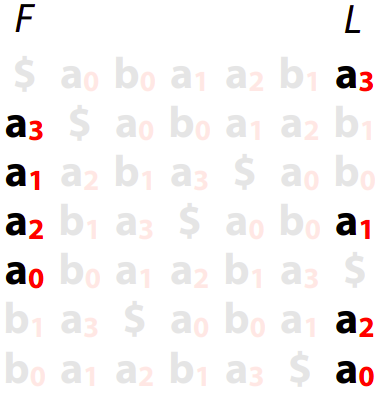
\includegraphics[width=100px]{./img/BWT_2.png}
		\caption{Burrows-Wheeler transformace last first mapping (LF). \cite{bw_transform}}
		\label{fig:bw_transform_lf}
\end{figure}

\noindent
Zpětné získání řetězce je znázorněno na obrázku \ref{fig:bw_transform_inverse}. L sloupec je řetězec který je výstupem BW transformace. F sloupec je snadné na základě L sloupce odvodit. Jelikož platí pravidlo, že počet jednotlivých znaků je stejný, stačí je pouze přemístit do F sloupce a seřadit podle abecedy. Dále s využítím LF je řetězec získán zpět. Jako první se vezme přidaný znak \$. Ve stejném řádku ve sloupci L se nachází $a_0$ . To znamená že řetězec začíná \$ a. Algoritmus pokračuje s $a_0$ v F sloupci. Ve stejném řádku v L sloupci je $b_0$. $b_0$ je přidáno do řetězce a pokračuje až do doby než by byl opět znak \$. 


\begin{figure}[H]		
		\centering
		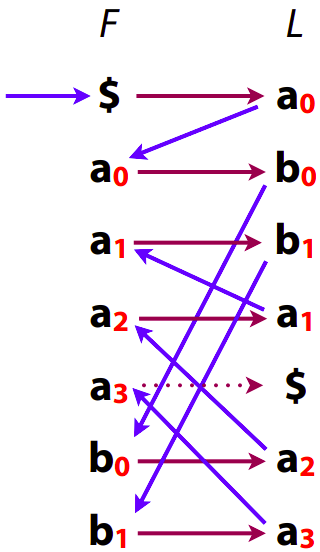
\includegraphics[width=80px]{./img/BWT_3.png}
		\caption{Burrows-Wheeler transformace zpětné získání původního řetězce. \cite{bw_transform}}
		\label{fig:bw_transform_inverse}
\end{figure}

\noindent
Díky vztahu mezi F a L sloupcem je možné vyhledávat daný řětezec (zobrazeno na obrázku \ref{fig:fm_index}). Například vyhledávány řetězec bude $P = aba$. Při pohledu do F sloupce jsou nalezeny všechy sloupce začínající $a$, následně v L sloupci ve stejných řádcích jsou nalezeny dva výskyty $b$. Již je získán sufix $ba$, který existuje. Pokračuje se dále na řádky, které začínají právě nalezenými $b$. V sloupci L pro dané řádky jsou nalezna $a$. Řětezec $P = aba$ se v textu vyskytuje. 

\begin{figure}[H]
		\centering
		\begin{subfigure}[t]{.4\textwidth}
			\centering
			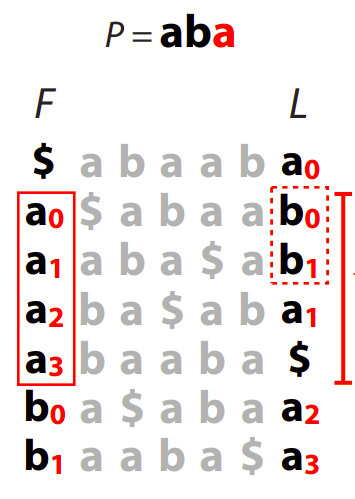
\includegraphics[width=100px]{./img/FM_index_1.png}
		\end{subfigure}
		%
		\begin{subfigure}[t]{.4\textwidth}
			\centering
			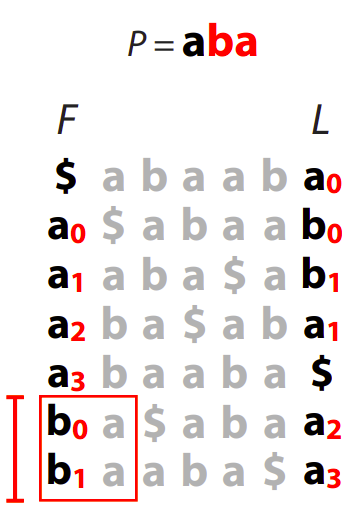
\includegraphics[width=100px]{./img/FM_index_2.png}
		\end{subfigure}	
		\caption{FM index - získání prefixu. \cite{bw_transform}}
		\label{fig:fm_index}
\end{figure}







\subsection{bordel}

FM index (Full-text minute-space) 
Přestože je tento vyhledávácí prostor velký , mnoho jeho částí může být přeskočeno (odřezáno) bez ztráty citlivosti
V praxi prořezávací strategie jako je dvojí indexování a obousměrné BWT usnadňuje v In practice, pruning strategies such as double indexing and bidirectional Burrows-Wheeler transform (BWT) facilitate very efficient untapped alignment of short reads.

 It is particularly good at aligning reads of about 50 up to 100s or 1,000s of characters, and particularly good at aligning to relatively long (e.g. mammalian) genomes.
  Bowtie 2 supports gapped, local, and paired-end alignment modes.

Note that SOAP2 and Bowtie do not permit gapped alignment of unpaired reads.

 We extracted a random subset of 1 million reads from each and aligned them with BWA-SW and Bowtie 2. We did not align with Bowtie, BWA or SOAP2 because those tools are designed for shorter reads.
Bowtie už je překonanej nejenom Bowtie2 ale i BWA.
Bowtie2 je podle studie znatelně lepší než Bowtie, SOAP2.
tyhle výsledky jsou na syntetických readech


pak tam máš parametry 

a jak dlouhý chceme simulovat ready? 

Výstupy se čtou ve formátu FASQ a zarování ve formátu ALN. 
ART může také generovat zarovnávání ve formátu SAM nebo UCSC BED
ART lze použít společně se simulátory varient genomů VarSim 
\\
to je odtud %https://www.niehs.nih.gov/research/resources/software/biostatistics/art/index.cfm
454 sekvenování je pyrosekvenování, které cycklicky testuje přítomnost každého ze čtyř nukleotidů DNA (T, A, C, G)


TODO nekam dopsat? musí se brát v potaz že z toho generátoru nikdy nebudou data taková jako reálná.. realná budou horší 


SAM Sequence Alignment Map format), respektive jeho binárně
komprimovaná verze BAM (z angl. Binary Alignment Map format).


\chapter{Implementace}
\section{Popis problému}
máme krátkou délku
že read který dostáváme jsou 250 bp dlouhé a jeden gen může být dlouhý 14738 bp
s tím že jednotlivé ready se nám tedy mohou překrývat- tohle si nejsem jistá jestli se můžou překrývat
můžou tam být chyby

teoreticky mám maximálně dvě možné alely s jednoho souboru, ale nemusím mít ani jednu 

pak by se tam dala přidat heurestika že bych brala známe haplotypy

Možná pak ještě pracovat s pravděpodobností výskytu daného genu

možná by se pak ještě dalo kolik readů tam bylo zarovnaných- ale to je blbost protože tam mám ready z několik genů ne jen z toho jednoho 

TODO jen by mě teda zajímalo jak to bere ten bowtie jestli když mu podšoupnu celej ten gen tak jestli se to snaží zarovnat vzhledem k celýmu geno jako takovýmu nebo to bere postupně podle alel.. 
po celym genomu by to asi bylo lepší protože pak by se dalo líp vyřešit to pokrytí 

jenže bowtie může klidně někam zarovant tam kam to ve skutečnosti napatří protože tam hledá třeba backtracking a nebo vložení a smazaní chybu


asi sem dopsat že i ty alely pro jeden gen můžou být různě dlouhé protože tam probíhají mutace

\section{Referenční geny}
Referenční geny byly převzaty z IPD-KIR \cite{imgt_hla_database} konkrétně soubory ve formátu $fasta$ uloženy ve stejnojmené složce. Jednotlivé soubory jsou pojmenovány genem, který obsahují např. $KIR2DL1\_gen.fasta$. Každý soubor představuje všechny dostupné alely konkrétního genu. Jedinou vyjímku tvoří soubory $KIR\_gen.*$, které obsahují všechny geny a navíc i pseudogeny. 
\\
\\
Kromě souborů $*\_gen.fasta$ obsahuje složka $fasta$ také soubory $*\_prot.fast$ a $*\_nuc.fasta$. Soubor $\_gen.fasta$ obsahuje informace o celých genech. Oproti tomu $\_nuc.fasta$ obsahuje nucleotidy, tedy pouze exony bez intronů. Soubor $*\_prot.fast$ obsahuje sekvence proteinů, které vznikly z RNA. 
\\
\\
TODO takže mě by ve finále mělo zajímát to nuc? 
\\
\\
TODO: KIR\_gen.fasta  includes the DNA sequence for all alleles, which have genomic sequences available.
\\
\\
TODO sem asi dodat ty věci ohledně dat z nemocnice

\section{Návrh systému}
Systém byl navržen jako modulární, díky tomu je možná jednoduchá náhrada jakékoliv jeho části. 
\\
\\ 
Vše začíná získáním dat pro která má být vyhodnoceno, které KIR alely obsahuje. Buď je možné dostat přímo data z Fakulní nemocnice čí biomedicínského centra. To jsou data na kterých bude prováděna verifikace nástroje. Druhou možností je data vyrobit. Na těchto datech byl nástroj vyvíjen a laděn. Data mohou být vyrobena ručně nebo je lze vyrobit za pomoci programu. V dalším kroku musí být haplotyp "rozbit" do podoby jako by vyšel ze sekvenátoru. Rozdělí se na ready a vytvoří s v něm chyby. To se provádí za pomoci nástroje ART.
\\
\\
V následující části jsou získaná data, tedy ready, zarovnána na referenční genom pomocí nástroje Bowtie. Nakonec je zarovnání vyhodnoceno a rozpoznáno o jaké alely genů se pravděpodoně jedná. Vyhodnocení je rozděleno do několika experimentů. Pro zjednodušení práce s výsledky je doplněn krok, kdy jsou názvy alel podle pořadových čísel nahrazen na názvy alel podle jejich skladby.

\begin{figure}[H]
		\centering
		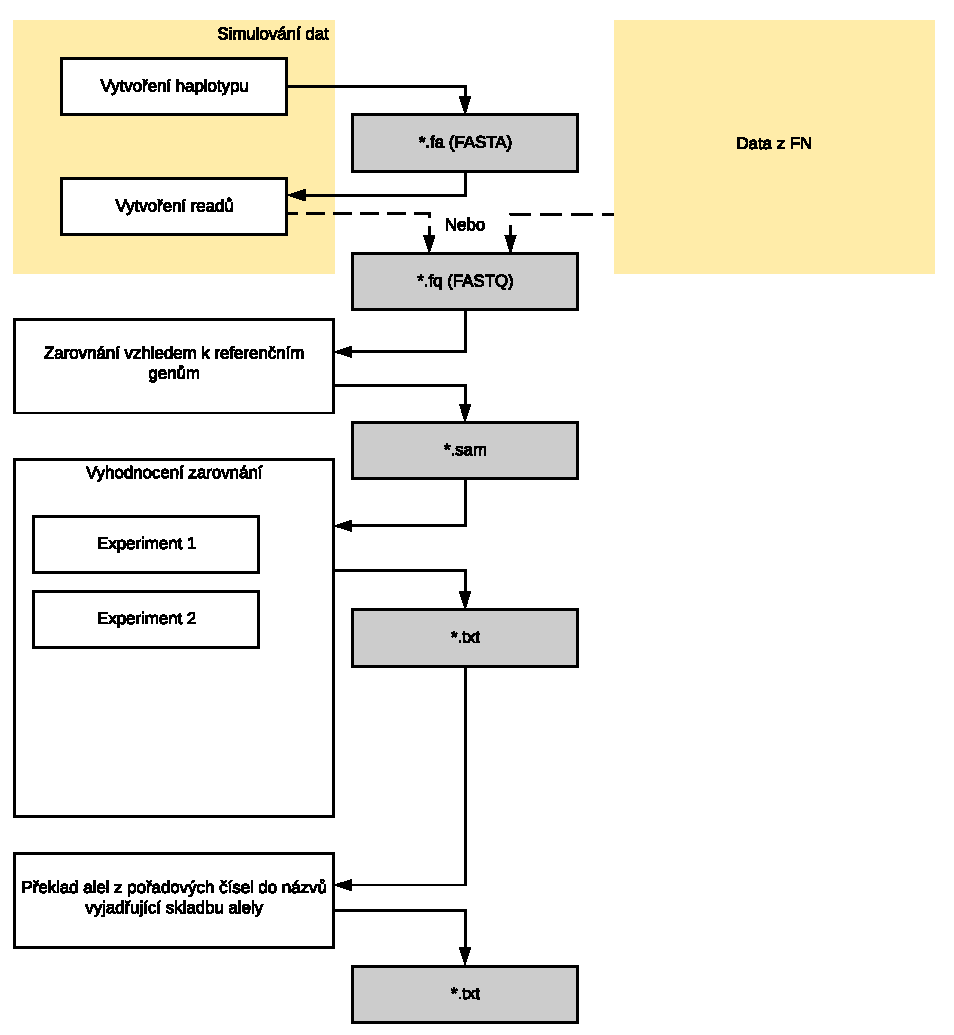
\includegraphics[width=\textwidth]{./img/navrh_systemu.pdf}
		\caption{Návrh systému. TODO to vyhodnoceni chce předělat. }
		\label{fig:navrh_systemu}
\end{figure}

\section{Použité programové prostředky}
\subsection{Python}
Program byl navržen a implementován na operačním systému Linux za použití především programovacího jazyku Python. 
 Pro spuštění programu je nutné mít nainstalovaný Python ve verzi 3.6.
\subsubsection{Biopython}
Biopython je sdružení vývojářů, kteří vytváří volné dostupné python nástoje vhodné pro výpočty v molekurární biologii. Biopython se snaží zjednoduší použití pythonu pro výzkum bioinformatiky. Mimo jiné umí pracovat s formáty souborů, které se využívají v bioinformatice jako je například BLAST nebo Fasta  
\\
\\
TODO
biopython jsem zatím ještě nepoužila
Instalaci jde provést pip install biopython
tak to vypadá že i ten biopython umí aligned a že to dělá přes to Burrows wheeler aligner 

\subsection{Bordel}
gen - jsou informace o celých genech, resp. jejich sekvencích, kdežto v nuc informace o nukleotidech - tedy jenom o exonech bez intronů, které při přepisu nehrají roli, tudíž se stává, že v nuc jsou stejné sekvence pro různé alely (jsou různé na třetí úrovni v názvu) - tím pádem je třeba zase se zkusit nějak vypořádat s podobností jednotlivých sekvencí

podobnost sekvencí je základním kamenem úrazu při identifikaci KIR a ta největší výzva při Vaší práci :)

gen obsahuje transkribované části bolasti přímo kódujícící pořadí aminikyselin proteinu (exony) i oblasti nekodující (introny), 

Co znamená konec 3 a konec 5? 
\\
\\
TODO takže mě by ve finále mělo zajímát to nuc? Co dostanu z nemocnice za data? Poprosit o poslání. 



\section{Modulové jednotky programu}
Vše potřebné pro samotný běh programu obstarává skript $run.py$ spolu s nastavením v souboru $config.py$. Skript $tun.py$ postupně pouští jednotlivé moduly. Díky nastavení v $config.py$ je možné si zvolit spuštění jen některých modulů. Například pouhé vytvoření testovacích dat nebo pouze jejich zarovnání a v neposlední řádě pouštět vyhodnocování zarovnávaných dat.

\subsection{Config}
S konfiguračním souborem \textit{config.py} jsou spojeny všechny skripty a obsahuje jejich veškerá nastavení. Jak již bylo zmíněno je možné pomocí tohoto nastavení spustit jednotlivé moduly. Jedná se především o položky \textit{CREATE\_READS}, která udržuje informaci o spuštění vytvoření syntetických readů. \textit{ALIGN} starající se o spuštění zarovnání a \textit{EVALUATE}, která řídí spuštění vyhodnocení zarovnání. Důležitou položkou v configu jsou cesty ke zdrojovým a výstupním složkám. Dalším nastavením je obsah haplotypu při případném vygenerování testovacích dat.
\\
\\
Pro urychlení běhu celého programu je v případě zmiňovanných referenčních genů možné použít poze soubor \textit{KIR\_gen.fasta}. Nastavení configu je jednoduché a to, nechat složku kam ukazuje \textit{REFERENCE\_KIR\_GENS\_FOLDER} prázdnou a položku \textit{REFERENCE\_KIR\_GENS\_FOLDER} nechat ukazovat na soubor \textit{KIR\_gen.fasta}.

\subsection{Simulování dat}
TODO to automatický vytváření mám možná trošku neefektivně , ale nevím jestli to úplně vadí nebo ne? 
třeba můžu napsat, že to nebylo stěžejní cíl práce tak že to vím, ale že už jsem to pak neupravovala, nebo to mám přepsat? Jako to přepsání asi bude rychlí
TODO hlavně mám v nastavení to kir gen folder a pak reference kir gens pseudogen file
TODO hele zkontroluj si v kodu jestli si náhodou někam napsala ručně to tvý \_gen.fasta
TODO možná že napsat že tahle chyba pro mě byla přínosem a tak pro někoho kdo se tím chce víc zabívat tak by to pro něj mohlo být také přínosem se podívat na to co mu to vlastně vyhazuje, je to experiment neni to program do praxe.

TODO no a tady zase nevím jestli to dělám dobře nebo ne protože já natahuju všechny ty soubory a přitom by mi vlastne stačil jedno a výhoda toho by byla že by to netrvalo tak dlouho, jako vždycky můžu dát do tý složky na referenční geny jen jeden soubor.. tak záleží co chci.. takhle tam teoreticky můžu strkat i víc těch referenčních genů a třeba koukat na který se to hodí víc nebo to porovnávat mezi sebou
i to jak se třeba chovají
tak nevím jestli někam třeba přidat sekci jak se vypozorovalo jak se chová bowtie třeba?
\\
\\
O simulování dat se stará skript \textit{create\_syntetic\_reads.py} a je rozděleno na dva kroky: vytvoření haplotypů a vytvoření readů. Mezi těmito dvěma fázemi vzniká soubory s příponou \textit{.fa}. Každý tento soubor obsahuje právě jeden KIR haplotyp. Tyto haplotypy jsou následně použíty jako vstupní soubor pro vytvoření readů, které se provádí za pomocí nástroje ART. Pro vytvoření haplotypů je volán skript \textit{create\_haplotype.py}, který vytvoří haplotypy na základě nastavení v configu pod položkou \textit{HAPLOTYPES} a za pomoci referenčních genů ve složce pod položkou \textit{REFERENCE\_KIR\_GENS\_FOLDER}. Vytvoření probíhá obdobně jako je popsáno níže u ručního vytvoření testovacího haplotypu. Výsledné haplotypy jsou uloženy do adresáře z configu \textit{HAPLOTYPE\_FOLDER}. Výstupem modulu \textit{create\_syntetic\_reads} je soubor s příponou \textit{.fq}, který by měl odpovídát formátu dat z nemocnice případně biomedicínského centra. Výstupní soubory jsou uloženy do složky pod promněnou \textit{READS\_FOLDER}.
\\
\\
\textbf{Ruční vytvoření testovacího haplotypu} lze udělat následujícím způsobem. V prvním kroku je vybrán gen, který je žádoucí vložit. V referenčních genech je vybrán jeho soubor a v tomto souboru je nalezena konkrétní alela. Někdy je možná najít shoda kdy se alely liší jen v konečné fazí jejich označení a v haplotypu je pouze první 5 čísel. S tímto jevem je možné se setkat například v případě alely 3DL3: 00402. V tomto případě může být vložena jakákoli z těchto alel. Vkladaná alela musí být vložena včetně její hlavičky tedy: \textit{>KIR:KIR00138 \: KIR3DL3*0040201 \: 12390 \: bp}. Je možné se setkat z genem, který se mezi soubory nenachází. Může se jednat například o pseudegen. Tyto geny je možné nalést v souboru \textit{KIR\_gen.fasta}, který obsahuje všechny geny pro které je známá jejich sekvence. Dalším způsobem vytvoření haplotypu je právě využítí souboru \textit{KIR\_gen.fasta}, díky čemuž je záskán stejný výsledek za použítí jen jednoho souboru. 
\\
\\
TODO když vytvářím gen tak tam dávám i tu hlavičku, bez ní mi Art totiž vytvořilo prázdný a navíc pan Fatka když mi posílal tu testovací tak to tam taky měl.. a pak mi bowtie píše magic number či co 
Myslím že pan Fatka mi poslal \textit{\_gen}
TODO jak je vlastně možný že mi tam vzniknou mezery s tím že nějakej gen není v haplotypu tak tam budu mít mezeru - jak je to v těch realných datech?
Nebo já jinak fakt nevím jak se identifikuje že tady je tenhle gen a tady je jinej gen?  

\subsection{Zarovnání vzhledem k referenčním genům}
Zarovnávání obstarává skript \textit{alignment\_reads\_to\_reference.py} s pomocí nástroje Bowtie. V nastavení je nutné vyplnit \textit{BOWTIE\_HOME\_DIRECTORY} podle umístění nástroje Bowtie na konkrétním počítači. V prvním kroku jsou vytvořeny bowtie indexy, které je možné použít na příč běhy, proto je v nastavení položka \textit{BOWTIE\_BUIL\_INDEX}, díky které je možné toto vytvoření povolit nebo zakázat. Bez vytovřených indexů, tedy indexů z minulých běhů, ale bowtie nebude zarovnávat. Bowtie vytváří indexy na základě obsahu složky \textit{REFERENCE\_KIR\_GENS\_FOLDER}. V dalším kroku jsem načteny všechny ready ze složky uvedené v \textit{READS\_FOLDER} a nasledně je na ně puštěn nástroj Bowtie. Tady je nutné aby byli ready paired end a to tedy aby se vyskytovali dvakrát jednou z \textit{1} na konci a podruhé s \textit{2}. V základu tento předpoklad zajistí správné nastavení ARTU, který je takto nastaven. Výstupní soubory jsou ve formátu \textit{.sam} a jsou umístěny dle položky \textit{ALIGMENT\_FOLDER} v nastavení. 

\subsection{Vyhodnoceni zarovnání}
\subsubsection{Experiment3}
asi smazat experiment 2 udělat z něj experiment 1 a pak udělat experiment 3
a tam je pak problém že mi to napíše i víc alel který tam můžou být takže kde je pak ta hranice kdy už nee
a navíc ten konec ty alely kolikrát neni specifikovanej ..
a podle toho co mi tam vychází tak je to po genech určitě blbost dělat protože twn bowtie se to snaží někam dát za každou cenu.

Já jsem to možná všechno dělala zbytečně moc složitě i to vytváření haplotypu, ten zbytek se dá zahladit tak, že prostě se tam dá vždycky jen ten jeden soubor .. že v těch referenčních genech tam nechá jenom to jedno pro který to bude chtít zarovnat zrovna 

\subsubsection{Experiment1}
	Počítání jen pokrytí za použití pysam.coverage či co 
	Klidně tam nějake graf algoritmu, hodí se to sem? 
	nevím jestli se nějak víc šťourat v těch bowtie nastavení.. u artu to nemá smysl protože tam se hlavně musím držet toho aby byli co nejvíc podobný těm z němocnice
	
TODO2: tenhle přístup mi nepřijde špatný, ale je nutno se zamyslet nad podobností alel a jak této informace využít, zkusit nějakou formu seskupování či identifikaci rozdílů alel a na základě jejich pokrytí (právě třeba maxima) rozhodovat či tak nějak něco

TODO jak je možné žé různé alely pro jeden gen mohou být různě dlouhé?
TODO2jedná se o různé varianty genu - mutace, chcete-li, tudíž tam mohlo docházet k insertům, deletům apod. a tudíž délka je jiná

\subsubsection{Experiment2}
rozdil oproti experimentu jedna je že jsem vzala jen KIR\_gen kde jsou všechny alely a tam to vypadá že to docela funguje



zkoušela jsem v pythonu přes pysam.depth, zkusit nějaký odhad na alely. Tak, že jsem zkusila vzít ty, které mají největší pokrytí. Brala jsem v úvahu i že každá alela je různě dlouhá, takže jsem to brala v procentech vzhledem k velikosti alely.  Zkrátka přijde mi, že to moc nefunguje, ale všimla jsem si takové zvláštnosti, že kolikrát se celý gen pohybuje kolem 99 procent pokrytí

\subsection{Překlad alel}
Při použití Bowtie vyvstal problém kdy jsou výsledné alely pojménovány pořadovým čísel jak byli objeveny nikoli názvem vyjadřující jejich skladbu. Proto vznikl modul překlad alel z pořadových čísel do názvů vyjadřující skladbu alely obsahující skript \textit{renaming\_alels\_result.py}, který projde všechny soubory ve složce pod proměnou \textit{RESULT\_FOLDER} a nahradí pořadová čísla příslušným názvem. Nakonec nahradí původní soubor, takto upraveným souborem.

\subsubsection{Mimo}
tenhle přístup mi nepřijde špatný, ale je nutno se zamyslet nad podobností alel a jak této informace využít, zkusit nějakou formu seskupování či identifikaci rozdílů alel a na základě jejich pokrytí (právě třeba maxima) rozhodovat či tak nějak něco


podobnost sekvencí je základním kamenem úrazu při identifikaci KIR a ta největší výzva při Vaší práci :)

About 80 procent of the exons on each chromosome are < 200 bp in length.

Když bych chtěla dělat podobnost textů tak se dá dělat hamingova vzdálenost. Vpodstatě vezmu dva řětězce a spočítám kolik mezi sebou mají rozdílů
- ale to je takový divný protože tam může být podobnost třeba posunutá ..

Levenshteinova metoda je o něco složitější. Jde o jeden z nejpoužívanějších algoritmů
pro zjištění vzdálenosti textových řetězců. Vyjadřuje podobnost/rozdílnost dvou textů na
základně počtu změn, které je potřeba udělat, abychom z jednoho řetězce dostali druhý.
Existují dvě hlaví varianty této metody - první, jednodušší a starší metoda je založená
na počtu úprav, které je nutno v řetězci provézt, abychom získali dva stejné řetězce.
Závisí tedy na počtu vložení, smazání nebo substituci. Ve své nejjednodušší podobě tento
algoritmus známý již přes čtyřicet let spočítá počet vložení, nahrazení a smazání nutných
k této transformaci
Druhá metoda je poněkud chytřejší a počítá i se složitostí daných operací, což ji dělá
realističtější, ale za to náročnější na výpočty.
- tady se dají řešit i ty posuny a tohle

Možná se dá ještě počítat frekvence výskytu jednotlivých znaků - ale máš 4 tak nevím jak hodně to je prokazatelný

TODO nikde jsem se nedočetla jak to přesně bere ten bowtie? Jestli zarovnává každou alelu v souboru zvlášť nebo dohromady? 
\\
\\
TODO zmínit někde běhy programu? Jako ono ten Bowtie běží celkem fest pomalu
\\
\\
TODO nevím jestli je úplně dobře že mám číslování stránek na obsahu a že mit o začíná od 6?
\section{Nastavení ART a bowtie}

pair end
250 dlouhy ready
misto MSv3 pouzit MSv1 protoze tak budou i data co dostanu
-f 100 pokryti 100
-na značí že nemá vytvořit soubor zarovnání
\chapter{Vyhodnocení výsledků a jejich srovnání}
\chapter{Závěr}
V práci bylo řešeno 

V teoretické části byli popsány a rozbrány Geny 

V realiziační části byl navržen a implementován program v jazyce Python 

Parametry ARTU byli nastaveny na základě dat z FN protože používají zrovna tenhle sekvenátor

Testování bylo prováděno na syntetických readech a následná validace byla provedena na datech z FN

Do budoucna by to chtělo co?

\chapter{Výkladový slovník pojmů a zkratek}

\begin{labeling}{alligator}
	\item [WHO] World health organization, světová zdravotnická organizace
	\item [ČNRDD] Český národní registr dárců kostní dřeně
	\item [MHC] Major histocompatibility complex, genetický systém	
	\item [HLA] Human leucocyte antigen, podskupina MHC
	\item [KIR] Killer imunoglobilin like-receptor, skupina genů
	\item [NK] Natural killer, buňka imunitního systému
	\item [DNA] Deoxyribonukleová kyselina; dvoušroubovice, která obsahuje páry bází C, G, A, T 
	\item [RNA] Ribonuklové kyselina; obsahuje báze C, G, A, U; šablona přímo pro vytvoření proteinů; hlavní funkcí zajištění překladu DNA do struktury proteinů (DNA -> mRNA -> rRNA -> tRNA -> RNA) 
	\item [Báze] nukleové báze; A - Adenin, C - Cytosin, G - Guanin, T - Thymin
	\item [bp] base pair; jeden z párů A - T nebo C - G
	\item [kb] kilobase 1 kb = 1000 bp
	\item [ART] nástroj na vytváření syntetických readů
	\item [Bowtie] nástroj na zarovnání readů proti referenčním genům
	\item [SAM] Sequence Alignment/Map; Formát souboru na uložení zarovnání
	\item [BAM] Binární verze souboru SAM
	\item [Fenotyp] adwda
	\item [Genotyp] adawwd
\end{labeling}


TODO tímhle si nejsem moc jistá tak jsem to pochopila je to dobře? DNA -> mRNA -> rRNA -> tRNA -> RNA
\\
\\
TODO co ty formáty souboru?

fenotyp tyhle kraviny
Genotyp pro danou chromozomální oblast se pak u většiny lidí skládá ze dvou haplotypů).
genom kompletní sekvence daného organismu

\textbf{DNA (Deoxyribonukleová kyselina)} \\ 
 - dvoušroubovice, která obsahuje páry bází C, G, A, T \\


obojí obsahuje nukleotidy bází? 
Rozdíl mezi DNA a RNA
DNA dvoušrobovice, která obsahuje páry bází - C G A T, kdežto RNA je již šablona přímo pro vytvoření proteinů takže jedna půlka šroubovice bez intronů. 
Hlavní funkcí RNA je zajištění překladu genetického kódu (DNA) do struktury proteinů
nejdřív je DNA  mRNA, rRNA tRNA RNA

Co znamená konec 3 a konec 5? 

% 
% PRO ANGLICKOU SAZBU JE NUTNÉ ZMĚNIT
% CITAČNÍ STYL!
%
\nocite{*}
\bibliographystyle{csplainnatkiv}
{\raggedright\small
\bibliography{literatura}
}


\appendix
\chapter{Uživatelská dokumentace}
Program byl napsán a otestován za použití ART ve verzi MountRainier, Bowtie 2 ve verzi 2.4.1, Python ve verzi 3.6. Dále byla použita pytnovská knihovny pysam ve verzi 0.14. 
\\
\\
Následující postupy jsou uvedeny pro operační systém Linux a pro jiné operační systémy se mohou lišit. Veškeré nastavení aplikace probíhá pomocí souboru \textit{config.py}
\\
\\
\noindent
Parametry configu:
\begin{itemize}
	\item CREATE\_READS - Značí zda má být spuštěn modul vytvoření syntetických readů. Očekávaný hodnota je True nebo False.
	\item ALIGN - Značí zda má být spuštěn modul pro zarovnání readů vzhledem k referenčním genům. Očekávaná hodnota je True nebo False.
	\item EVALUATE - Značí zda má být spuštěno vyhodnocení zarovaných readů. Očekávaná hodnota je True nebo False.
	\item REFERENCE\_KIR\_GENS\_FOLDER - Referenční geny by měli obsahovat cestu k složce ve které se nachází referenční geny.
	\item REFERENCE\_KIR\_GENS\_PSEUDOGENS\_FILE - Dodatečný soubor, který se bude prohledávat v případě že gen nebude nalezen ve složce REFERENCE\_KIR\_GENS\_FOLDER. Typickým příkladem mohou být pseudegeny. 
	\item HAPLOTYPE\_FOLDER - Označuje cestu složky do které jsou ukládány vytvořené haplotypy. 
	\item HAPLOTYPES - Slovník, který definuje haplotypy podle obsahů genů. Na základě toho budou vytvořeny haplotypy.
	\item BOWTIE\_HOME\_DIRECTORY - Označuje cestu ke nástroji Bowtie.
	\item READS\_FOLDER - Označuje složku do které budou ukládany ready. Případně z které budou načítány.
	\item BOWTIE\_INDEX\_FOLDER - Označuje složku do které budou ukládány indexy z Bowtie. Případně z které budou načítány. 
	\item BOWTIE\_BUILD\_INDEX - Značí zda mají být vytvořeny Bowtie indexy. Pokud bude hodnota nastavena na False, musí být přítomny indexy z minulého běhu, jinak zarovnávání nebude fungovat. Očekávaná hodnota je True nebo False.
	\item BOWTIE\_THREADS - Počet vláken na která má být Bowtie spuštěn.	
	\item ALIGNMENT\_FOLDER - Označuje složku do které budou ukládány zarovnané ready. Případně z které budou načítány. 
	\item BAM\_FOLDER - Označuje složku na uložení BAM souborů.  
	\item RESULT\_FOLDER - Označuje složku do které budou uloženy výsledky vyhodnocení zarovnání.
\end{itemize}


\section{Spuštění programu}
Program je možné spustit z příkazové řádky pomocí příkazu \textit {python run.py}. Podmínkou fungování tohoto postupu je, že je třeba se nacházet v umístění skriptu. 

\section{Doporučená adresářová struktura pro data}
\begin{itemize}
	\item data
		\begin{itemize}
			\item alignments
			\item bam
			\item bowtie\_index
			\item haplotype
			\item reads
			\item result
		\end{itemize}
\end{itemize}

\section{Výstupy programu}
V případě tvorby vlastních haplotypů s doporučenou adresářovou strukturou najdeme ve složce \textit{haplotype} soubory s příponou \textit{.fa}. Každý soubor obsahuje jeden haplotyp.
Vytvořené ready se budou nacházet ve složce reads. Protože haplotypy jsou paired-end náleží každému haplotypu dva soubory s příponou \textit{.fq}. Jeden s \textit{1} na konci a druhý s \textit{2} na konci. 
V případě zarovnání mohou být výstupní soubory indexy ve složce \textit{bowtie\_index}. Kdy pro každý referenční gen je vytvořeno 6 souborů s příponou \textit{.1.ebwt}, \textit{.2.ebwt}, \textit{.3.ebwt}, \textit{.4.ebwt}, \textit{.rev.1.ebwt} a \textit{.rev.2.ebwt}. Výsledné zarování se pak nachází ve složce \textit{alignments} ve formátu \textit{.sam}. Vyhodnocení zarovnání se pak nacháze ve složce \textit{result} ve formátu \textit{.txt}

\chapter{Uživatelská dokumentace ART???}
\section{Nastavení ART a jeho spuštění}
tak jsem stáhla normálně nejnovější verzi z niehs.nih.gov a podle instrukcí co byli v souboru INSTAL dala % ./configure && make && make install

\subsection{pokus to nejak spustit}
Takze kdyz otebru hlavni readme tak mi to riká že tam jsou read me pro jednotlivy verze sekvenatoru ..

pak se to musí skompilovat 

./configure --prefix=\$HOME
	       	make
	       	make install	 
	 
teď mě zajímá ta ilumia tak podle readme ilumina tak můžu vlést do složky examples a tam pustit skript run\_test\_examples\_illumina.sh , tak tam jsou 4 příklady použití 
a pokud asi všechno dobře porběhne tak se mi zobrazí pár nových souborů ve složce examples.. 

FASTQ - *.fq data file s ready. pro paired-red simulator
*1.fq obsahuje data pro rvní ready a *2.fq rdu druhy ready

tohle nějak funguje
MSv3 tam musím dát abych to mohla dostat na délku readu 250 a p znaci ze to je paired.. 
tak se má používát MSv1
$art_illumina -ss MSv3 -sam -i amplicon_reference.fa -p -l 250 -f 10 -m 300 -s 10 -o moje_art_data$
Tohle používej:
$art_illumina -ss MSv1 -sam -i amplicon_reference.fa -p -l 250 -f 100 -m 300 -s 10 -o moje_art_data$

\chapter{Uživatelská dokumentace Bowtie ??}
\section{Bowtie}
 a stáhla jsem to tady %http://bowtie-bio.sourceforge.net/tutorial.shtml
 po kliknuti na bowtie binary release.

na strance 25.4 je řečeno o hledání tch nejlepších zarovnání a je tam možnost --best ale že je dvakrát nebo třikrát pomalejší než normální mod.. a jde o to že najde první přijatelný a to označní kdežto při tom best prohledá co nejvíc a hledá to nejlepší i mezi těma přijatelnýma a to je pomalý.


tak jsem  to stáhla dala do složky a musela jsem teda nastavit proměnou prostředí 
export BT2\_HOME=$/home/kate/Dokumenty/FAV/Diplomka/existujicisw/bowtie2-2.4.1-linux-x86_64/$
pak jsem pustila tohle: 
\$BT2\_HOME/bowtie2-build \$ $BT2_HOME/example/reference/lambda_virus.fa lambda_virus$
a nakonec se mi vytvořili nějaký nový soubory lambda virus 1 atd.. v tom bowtie 2 adresáři

dělala jsemt o podle tohohle webovky %http://bowtie-bio.sourceforge.net/bowtie2/manual.shtml#getting-started-with-bowtie-2-lambda-phage-example



indexy
bowtie-build builds a Bowtie index from a set of DNA sequences. bowtie-build outputs a set of 6 files with suffixes .1.ebwt, .2.ebwt, .3.ebwt, .4.ebwt, .rev.1.ebwt, and .rev.2.ebwt. (If the total length of all the input sequences is greater than about 4 billion, then the index files will end in ebwtl instead of ebwt.)
 These files together constitute the index: they are all that is needed to align reads to that reference. The original sequence files are no longer used by Bowtie once the index is built.

\chapter{Používané soubory}
\subsection{FASTQ}

	    
	    aln\_start\_pos označuje počáteční pozicí v referenci sekvence, je vždy relativní vzhledem k vláknu referenční sekvence
	    To znamená že aln\_start\_pos plus (10) vlákno je odlišný od  aln\_start\_pos minus (-) vlákna.. ???? WHAT???
	    
		ref\_seq\_aligned je zarovnaná oblast referenční sekvence, která může být plus vlákno nebo mínos vlákno referenční sekvence
		ref\_seq\_aligned je zarovanný read, který je vždy ve stejné orientaci jako stejný read v odpovívajícím fastq suboru.  
		
		
			    
	    
	       	
		aln\_start\_pos is the alignment start position of reference sequence. aln\_start\_pos is always relative to the strand of reference sequence. That is, aln\_start\_pos 10 in the plus (+) strand is different from aln\_start\_pos 10 in the minus (‐) stand.  
	
		ref\_seq\_aligned is the aligned region of reference sequence, which can be from plus strand or minus strand of the reference sequence. 
		read\_seq\_aligned is the aligned sequence read, which always in the same orientation of the same read in the corresponding fastq file. 

SAM je standardní formát pro NG sekvence ready zarování
BED o tom tam nic neni jen 
NOTE: both ALN and BED format files use 0-based coordinate system while SAM format uses 1-based coordinate system.

pak jsou tady 4 doporučené použití
$art_illumina [options] -ss <sequencing_system> -sam -i <seq_ref_file> -l <read_length> -f <fold_coverage> -o <outfile_prefix>$
$art_illumina [options] -ss <sequencing_system> -sam -i <seq_ref_file> -l <read_length> -c <num_reads_per_sequence> -o <outfile_prefix>$
$art_illumina [options] -ss <sequencing_system> -sam -i <seq_ref_file> -l <read_length> -f <fold_coverage> -m <mean_fragsize> -s <std_fragsize> -o <outfile_prefix>$
$art_illumina [options] -ss <sequencing_system> -sam -i <seq_ref_file> -l <read_length> -c <num_reads_per_sequence> -m <mean_fragsize> -s <std_fragsize> -o <outfile_prefix>$
\subsection{FASTQ}
Sekvenační přístroje produkují data ve formátu FASTQ takže i ART musí logicky generovat tenhle formát.
Pokud jsou ready v páru tak je na konci .1
a druhý read z páru tam má .2 to jsem u těch svých přímo nenašla 

ale máš teda tři druhy single end, paired-end a matepair. 

FASTQ obsahuje obě základy sekvence ?? both sequence bases a kvality skore je to v následujícím formátu
@read\_id
sequence read
+
base quality scores je kódovany by ascii code of a single character, kde je kvalita rovná score to ascii code character minus 33. chápu proč tam je to -33 protže když se podíváš do asci tabulky tak je tam od 33 první normální znak jinakjsou tam divný .. 
takže třeba otazník je v asci na 63 takže -33 takže má ohodnocení kvality 30
jen by mě teda zajímalo v jakým sme intervalu? - je 45 v asci a nevím jestli to je teda od 0 do 100?  a teda nejvyšší číslo znamená nejkvalitnější a nejmenši míň kvalitní? Podle tý diplomky to tak je že čím vyšší číslo tím kvalitnější a většinou je to od 0 do 40 jen zřídka to překročí hodnotu 60, když je tam 10 tak to znamneá že jedna báze z deset je špatně.. když je tam 30 tak to znamená že jedna z 1000 je špatně.
já tam mám třeba F a to je 70.

example:
		@refid-4028550-1 
		caacgccactcagcaatgatcggtttattcacgat...
		+ 
%		????????????7?????<??>??=&?<<?-<?0?...

ALN - zarovnání readů
zase *1.aln pro první a *2.aln pro druhý
soubor je rozdělen na hlavičku a body část
obsahuje hlavičku a v tý hlavičce je jakým příkazem byl soubor vygenerován a reference na sequnce id a jejich délku
@CM tag pro příkaz a
@SQ pro reference sequence
Hlavička vždycky začíná s 
%##ART a končí s ##header end

		HEADER EXAMPLE

%		##ART_Illumina  read_length     35
%		@CM     ../art_illumina -i ./testSeq.fa -o ./single_end_com -l 35 -f 10 -sam -rs 177
%		@SQ     seq1    7207
%	       	@SQ     seq2    3056
%		##Header End
		
v body jsou všechny zarovnání 
%		>ref_seq_id	read_id	aln_start_pos	ref_seq_strand
%	       	ref_seq_aligned
%	       	read_seq_aligned 

\subsection{SAM a BAM}
1. název readu který je zarovnáván

2. Sum of all applicable flags. Flags relevant to Bowtie are:
součet všechn aplikovaných (příslušných flags). Flagy relevantní k bowtie jsou: 
1 - read je jeden z páru
2 - zarovnání je one z paired proper (The alignment is one end of a proper paired-end alignment)
4 - read má reported alignments
8 - read je jeden z páru a má reportovaný zarovnání
16 - zarování je obrácená reference vlákna
32 - The other mate in the paired-end alignment is aligned to the reverse reference strand
64 - read je mate 1 in a pair
128 - read je mate 2 in a pair

Thus, an unpaired read that aligns to the reverse reference strand will have flag 16. A paired-end read that aligns and is the first mate in the pair will have flag 83 (= 64 + 16 + 2 + 1).

3. jméno referecnce ze které zarování patří
4. 1-based offset into the forward reference strand where leftmost character of the alignment occurs 1-based odszaneí v následující referenci 
5. kvalita mapování
6. CIGAR reprezentace zarovnání
7. název reference kde je zarovnán kamarád 
8. 1-based zarování ofsetu k nálsedující refenrenci 
9. Odvozená délka fragmentu. Velikost v závoru je že se mate nachází předtím. 0 že jsem nezarovnali mate
10. read sekvence
11. ASCII encoded read kvalita, stejné jako u FASTQ
12. optional pole
\end{document}
